 \documentclass[a4paper]{article}
\usepackage{vntex}
%\usepackage[english,vietnam]{babel}
%\usepackage[utf8]{inputenc}

%\usepackage[utf8]{inputenc}
%\usepackage[francais]{babel}
\usepackage{a4wide,amssymb,epsfig,latexsym,multicol,array,hhline,fancyhdr}
\usepackage{booktabs}
\usepackage{amsmath}
\usepackage{lastpage}
\usepackage[lined,boxed,commentsnumbered]{algorithm2e}
\usepackage{enumerate}
\usepackage{color}
\usepackage{graphicx}							% Standard graphics package
\usepackage{array}
\usepackage{tabularx, caption}
\usepackage{multirow}
\usepackage[framemethod=tikz]{mdframed}% For highlighting paragraph backgrounds
\usepackage{multicol}
\usepackage{rotating}
\usepackage{graphics}
\usepackage{geometry}
\usepackage{setspace}
\usepackage{epsfig}
\usepackage{tikz}
\usepackage{listings}
\usepackage{xcolor}
\usetikzlibrary{arrows,snakes,backgrounds}
\usepackage{hyperref}
\hypersetup{urlcolor=blue,linkcolor=black,citecolor=black,colorlinks=true} 
%\usepackage{pstcol} 								% PSTricks with the standard color package

\newtheorem{theorem}{{\bf Định lý}}
\newtheorem{property}{{\bf Tính chất}}
\newtheorem{proposition}{{\bf Mệnh đề}}
\newtheorem{corollary}[proposition]{{\bf Hệ quả}}
\newtheorem{lemma}[proposition]{{\bf Bổ đề}}

\everymath{\color{blue}}
%\usepackage{fancyhdr}
\setlength{\headheight}{40pt}
\pagestyle{fancy}
\fancyhead{} % clear all header fields
\fancyhead[L]{
 \begin{tabular}{rl}
    \begin{picture}(25,15)(0,0)
    \put(0,-8){
\includegraphics[width=8mm, height=8mm]{logoITSGUsmall.png}}
    %\put(0,-8){\epsfig{width=10mm,figure=hcmut.eps}}
   \end{picture}&
	%\includegraphics[width=8mm, height=8mm]{hcmut.png} & %
	\begin{tabular}{l}
		\textbf{\bf \ttfamily Trường Đại học Sài Gòn}\\
		\textbf{\bf \ttfamily Khoa Công Nghệ Thông Tin}
	\end{tabular} 	
 \end{tabular}
}
\fancyhead[R]{
	\begin{tabular}{l}
		\tiny \bf \\
		\tiny \bf 
	\end{tabular}  }
\fancyfoot{} % clear all footer fields
\fancyfoot[L]{\scriptsize \ttfamily Bài tập lớn môn Phát triển phần mềm mã nguồn mở - Niên khóa 2023-2024}
\fancyfoot[R]{\scriptsize \ttfamily Trang {\thepage}/\pageref{LastPage}}
\renewcommand{\headrulewidth}{0.3pt}
\renewcommand{\footrulewidth}{0.3pt}


%%%
\setcounter{secnumdepth}{4}
\setcounter{tocdepth}{3}
\makeatletter
\newcounter {subsubsubsection}[subsubsection]
\renewcommand\thesubsubsubsection{\thesubsubsection .\@alph\c@subsubsubsection}
\newcommand\subsubsubsection{\@startsection{subsubsubsection}{4}{\z@}%
                                     {-3.25ex\@plus -1ex \@minus -.2ex}%
                                     {1.5ex \@plus .2ex}%
                                     {\normalfont\normalsize\bfseries}}
\newcommand*\l@subsubsubsection{\@dottedtocline{3}{10.0em}{4.1em}}
\newcommand*{\subsubsubsectionmark}[1]{}
\makeatother

\definecolor{dkgreen}{rgb}{0,0.6,0}
\definecolor{gray}{rgb}{0.5,0.5,0.5}
\definecolor{mauve}{rgb}{0.58,0,0.82}

\lstset{frame=tb,
	language=Matlab,
	aboveskip=3mm,
	belowskip=3mm,
	showstringspaces=false,
	columns=flexible,
	basicstyle={\small\ttfamily},
	numbers=none,
	numberstyle=\tiny\color{gray},
	keywordstyle=\color{blue},
	commentstyle=\color{dkgreen},
	stringstyle=\color{mauve},
	breaklines=true,
	breakatwhitespace=true,
	tabsize=3,
	numbers=left,
	stepnumber=1,
	numbersep=1pt,    
	firstnumber=1,
	numberfirstline=true
}

\begin{document}

\begin{titlepage}
\begin{center}
TRƯỜNG ĐẠI HỌC SÀI GÒN \\
KHOA CÔNG NGHỆ THÔNG TIN
\end{center}
\vspace{1cm}

\begin{figure}[h!]
\begin{center}

\includegraphics[width=3cm]{logoITSGU.png}
\end{center}
\end{figure}

\vspace{1cm}

\begin{center}
\begin{tabular}{c}
	\multicolumn{1}{l}{\hspace{0,5cm}\textbf{{\Large \color{black} PHÁT TRIỂN PHẦN MỀM MÃ NGUỒN MỞ}}}\\
	~~\\

	\textbf{{\Large \color{black} Phát triển phần mềm Play Audio - Video}}\\

\end{tabular}
\end{center}

\vspace{3cm}
\begin{table}[h]
\begin{tabular}{rrl}
\hspace {5 cm} &\color{black} GVHD: & \color{black}Từ Lãng Phiêu\\
&\color{black} Sinh Viên: &\color{black} Nguyễn Bá Lợi - 3120560056\\
      &&\color{black} Trần Công Hùng -  3120410197\\
      && \color{black}Nguyễn Hoài Kha -  3120410228\\

\end{tabular}
\vspace{1.5 cm}
\end{table}

\begin{center}
{\footnotesize TP. HỒ CHÍ MINH, THÁNG 5/2024}
\end{center}
\end{titlepage}


\thispagestyle{empty}

\newpage
\tableofcontents
\newpage

%%%%%%%%%%%%%%%%%%%%%%%%%%%%%%%%%


%%%%%%%%%%%%%%%%%%%%%%%%%%%%%%%%%
\section{Giới thiệu đề tài}
    \hspace*{0.5cm}\Large Trong thời đại số ngày nay, việc làm việc với âm thanh và video đã trở nên phổ biến và quan trọng hơn bao giờ hết. Đặc biệt, việc phát audio và video không chỉ dành cho giải trí mà còn được ứng dụng rộng rãi trong nhiều lĩnh vực khác nhau như giáo dục, truyền thông và công nghệ thông tin. Trong bối cảnh này, nghiên cứu về các phần mềm được thiết kế từ ngôn ngữ Python để phát audio và video không chỉ mang lại sự linh hoạt và hiệu suất mà còn mở ra nhiều cơ hội cho phát triển ứng dụng đa phương tiện..

    \hspace*{0.5cm}\Large Ứng dụng sẽ được phát triển với giao diện đồ họa người dùng (GUI) thân thiện, cho phép người dùng dễ dàng thêm danh sách bài hát mà họ muốn nghe, hoặc có thể xoá những bài hát mà họ khuông muốn có trong danh sách. Ngoài ra người dùng có thể play video mà họ muốn phát bằng cách mở thư mục riêng có trên phần mềm. Bên cạnh đó ứng dụng còn có thể play với nhiều định dạng khác nhau như .mp3, .mp4, .flac, .wav, .aiff, .ogg, .mov, .avi. Ngoài ra người dùng còn có thể điều chỉnh âm lượng trên ứng dụng.

\newpage

\section{Cơ sở lý thuyết}
\subsection{Ngôn ngữ Python}
\subsubsection{Giới thiệu ngôn ngữ Python}
    \hspace*{0.5cm}\Large Python là ngôn ngữ lập trình cấp cao, hướng đối tượng, diễn giải với ngữ nghĩa động được phát triển bởi Guido van Rossum. Ban đầu nó được phát hành vào năm 1991. Được thiết kế để dễ sử dụng cũng như vui nhộn, cái tên "Python" là sự gợi nhớ đến nhóm hài kịch người Anh Monty Python. Python nổi tiếng là ngôn ngữ thân thiện với người mới bắt đầu, thay thế Java trở thành ngôn ngữ giới thiệu được sử dụng rộng rãi nhất vì nó xử lý phần lớn sự phức tạp cho người dùng, cho phép người mới bắt đầu tập trung vào việc nắm bắt đầy đủ các khái niệm lập trình hơn là các chi tiết nhỏ.

    \hspace*{0.5cm}\Large Python được sử dụng để phát triển web phía máy chủ, phát triển phần mềm, toán học và viết kịch bản hệ thống, đồng thời phổ biến cho Phát triển ứng dụng nhanh và là ngôn ngữ viết kịch bản hoặc kết dính để liên kết các thành phần hiện có vì cấu trúc dữ liệu tích hợp, cấp cao của nó, gõ động và ràng buộc động. Chi phí bảo trì chương trình được giảm bớt bằng Python do cú pháp dễ học và nhấn mạnh vào khả năng đọc. Ngoài ra, sự hỗ trợ của các mô-đun và gói của Python tạo điều kiện thuận lợi cho các chương trình mô-đun và tái sử dụng mã. Python là ngôn ngữ cộng đồng nguồn mở nên rất nhiều lập trình viên độc lập đang liên tục xây dựng thư viện và chức năng cho nó.
\subsubsection{Ứng dụng của Python}
\hspace*{0.5cm} Dữ liệu và trực quan hóa dữ liệu. Vì tương đối dễ học, Python đã được nhiều người không phải là lập trình viên như kế toán và nhà khoa học áp dụng cho nhiều công việc hàng ngày, chẳng hạn như tổ chức tài chính.
\begin{itemize}
    \item Phân tích dữ liệu và học máy: Python đã trở thành một công cụ không thể thiếu trong lĩnh vực khoa học dữ liệu. Với sức mạnh của các thư viện như NumPy, Pandas, và Matplotlib, Python cho phép các nhà phân tích dữ liệu thực hiện các phép tính thống kê phức tạp, tạo ra các biểu đồ trực quan, và xây dựng các mô hình học máy. Các thư viện như TensorFlow và Keras cung cấp cho lập trình viên các công cụ mạnh mẽ để phát triển và huấn luyện mô hình học máy, từ nhận diện hình ảnh đến dự đoán chuỗi thời gian. Python không chỉ là một ngôn ngữ lập trình, mà còn là một hệ sinh thái mạnh mẽ hỗ trợ cho việc nghiên cứu và ứng dụng trong lĩnh vực dữ liệu..
    \item Phát triển web: Python thường được sử dụng để phát triển back-end của trang web hoặc ứng dụng—những phần mà người dùng không nhìn thấy. Vai trò của Python trong phát triển web có thể bao gồm gửi dữ liệu đến và đi từ máy chủ, xử lý dữ liệu và giao tiếp với cơ sở dữ liệu, định tuyến URL và đảm bảo tính bảo mật. Python cung cấp một số khuôn khổ để phát triển web. Những cái thường được sử dụng bao gồm Django và Flask.Một số công việc phát triển web sử dụng Python bao gồm kỹ sư phụ trợ, nhà phát triển Python, kỹ sư phần mềm và kỹ sư DevOps.
    \item Tự động hoá và phát triển phần mềm: Python thường được sử dụng để phát triển back-end của trang web hoặc ứng dụng—những phần mà người dùng không nhìn thấy. Vai trò của Python trong phát triển web có thể bao gồm gửi dữ liệu đến và đi từ máy chủ, xử lý dữ liệu và giao tiếp với cơ sở dữ liệu, định tuyến URL và đảm bảo tính bảo mật. Python cung cấp một số khuôn khổ để phát triển web. Những cái thường được sử dụng bao gồm Django và Flask.Một số công việc phát triển web sử dụng Python bao gồm kỹ sư phụ trợ, nhà phát triển Python, kỹ sư phần mềm và kỹ sư DevOps.
    \item Tự động hoá và phát triển phần mềm: Python không chỉ là một ngôn ngữ lập trình mạnh mẽ, mà còn là một công cụ tuyệt vời cho việc tự động hóa các nhiệm vụ lặp đi lặp lại. Việc viết script trong Python giúp tự động hóa các quy trình như kiểm tra lỗi, chuyển đổi tệp, và loại bỏ các bản sao dữ liệu. Ngay cả những người mới bắt đầu cũng có thể sử dụng Python để tự động hóa các tác vụ đơn giản trên máy tính, như đổi tên tệp, tìm kiếm và tải xuống nội dung trực tuyến, hoặc gửi email theo lịch trình. Trong phát triển phần mềm, Python cũng hỗ trợ các tác vụ như kiểm soát bản dựng, theo dõi lỗi, và kiểm thử sản phẩm mới. Điều này giúp các nhà phát triển phần mềm tự động hóa các quy trình kiểm thử và đảm bảo chất lượng sản phẩm.

\end{itemize}
\subsubsection{Đặc tính của Python}
    \hspace*{0.5cm}\Large Python đang trở nên phổ biến trong cộng đồng lập trình nhờ có các đặc tính sau:
\begin{itemize}
    \item Ngôn ngữ thông dịch: Python được xử lý trong thời gian chạy bởi Trình thông dịch Python.
    \item Ngôn ngữ hướng đối tượng: Nó hỗ trợ các tính năng và kỹ thuật lập trình hướng đối tượng.
    \item Ngôn ngữ lập trình tương tác: Người dùng có thể tương tác trực tiếp với trình thông dịch python để viết chương trình.
    \item Ngôn ngữ dễ học: Python rất dễ học, đặc biệt là cho người mới bắt đầu.
    \item Cú pháp đơn giản: Việc hình thành cú pháp Python rất đơn giản và dễ hiểu, điều này cũng làm cho nó trở nên phổ biến.
    \item Dễ đọc: Mã nguồn Python được xác định rõ ràng và có thể nhìn thấy bằng mắt.
    \item Di động: Mã Python có thể chạy trên nhiều nền tảng phần cứng có cùng giao diện.
    \item Có thể mở rộng: Người dùng có thể thêm các mô-đun cấp thấp vào trình thông dịch Python.
    \item Có thể cải tiến: Python cung cấp một cấu trúc cải tiến để hỗ trợ các chương trình lớn sau đó là shell-script.
    
\end{itemize}
\subsection{Các thư viện sử dụng}
\subsubsection{Thư viện Pygame}
    \hspace*{0.5cm} Pygame là một thư viện của ngôn ngữ lập trình Python và là một tập hợp các mô-đun Python được thiết kế riêng để lập trình trò chơi. Pygame được viết bởi Pete Shinners thay thế cho chương trình PySDL sau khi quá trình phát triển dự án này bị đình trệ. Chính thức phát hành từ năm 2000, Pygame được phát hành theo phần mềm miễn phí GNU Lesser General Public License.

    \hspace*{0.5cm} Pygame có thể chạy trên nhiều nền tảng và hệ điều hành khác nhau. Với thư viện pygame trong Python, các nhà phát triển có thể sử dụng công cụ và chức năng mở rộng để tạo ra các trò chơi nhập vai ấn tượng. Bởi vậy, Pygame đang ngày càng phổ biến với nhà phát triển vì tính đơn giản, linh hoạt, dễ sử dụng.

    \hspace*{0.5cm} Các tính năng chính của Pygame bao gồm:
    \begin{itemize}
          \item Pygame sử dụng Simple DirectMedia Layer (SDL), một thư viện phát triển đa nền tảng cho phép các nhà phát triển có thể truy cập vào phần cứng máy tính như đồ họa, âm thanh và thiết bị đầu vào.
          \item Xây dựng các trò chơi trên nhiều nền tảng khác nhau như Windows, Mac, Linux thậm chí là cả các thiết bị di động
          \item Nhà phát triển có thể quản lý tất cả các yếu tố trong quá trình phát triển trò chơi. Đó có thể là các chức năng như xuất đồ họa, xử lý sự kiện, hoạt ảnh, hiệu ứng âm thanh và phát lại nhạc.
          \item API trực quan và dễ hiểu, hỗ trợ người mới sử dụng hay cả những nhà phát triển có kinh nghiệm đều có thể truy cập được.
          \item Tính đa phương tiện giúp nhà phát triển có thể ứng dụng để xử lí hình ảnh hay video, mô phỏng, công cụ giáo dục….
      \end{itemize}  

      \hspace*{0.5cm} Bạn có thể cài đặt Pygame thông qua pip, trình quản lý gói cho Python. Lệnh cài đặt thông thường là: pip install pygame.
\subsubsection{Thư viện Tkinter}
     \hspace*{0.5cm} Tkinter là một thư viện trong ngôn ngữ lập trình Python được sử dụng để tạo giao diện đồ họa người dùng (GUI). "Tkinter" là viết tắt của "Tk interface,", một toolkit đồ họa cung cấp các công cụ để phát triển giao diện người dùng.
     
      \hspace*{0.5cm} Tkinter là một phần của thư viện tiêu chuẩn của Python và đã được tích hợp sẵn trong hầu hết các cài đặt Python. Điều này giúp cho Tkinter trở thành một lựa chọn phổ biến cho việc phát triển ứng dụng với giao diện đồ họa đơn giản trong Python.
      
      \hspace*{0.5cm} Một số đặc điểm của Tkinter bao gồm khả năng tạo các thành phần giao diện như cửa sổ, nút, ô văn bản, và các widget khác để tương tác với người dùng. Tkinter cung cấp cả các sự kiện và phương thức để xử lý tương tác người dùng và thay đổi trạng thái của ứng dụng.

      \hspace*{0.5cm} Tkinter được cài đặt mặc định với Python, vì vậy không cần phải cài đặt bổ sung..
\subsubsection{OS}
     \hspace*{0.5cm} Thư viện os trong Python cung cấp các chức năng để tương tác với hệ điều hành, bao gồm truy cập vào các tệp và thư mục, thực thi các lệnh hệ thống, và nhiều hơn nữa.
     
     \hspace*{0.5cm} Các tính năng chính của thư viện OS bao gồm:
      \begin{itemize}
          \item Kiểm tra sự tồn tại của tệp.
          \item Tạo thư mục mới.
          \item Thao tác với thư mục:
          \begin{itemize}
              \item Lấy thư mục hiện tại.
              \item Di chuyển thư mục.
              \item Xoá thư mục.
          \end{itemize}
          \item Thao tác với đường dẫn.
          \begin{itemize}
              \item Lấy đường dẫn tuyệt đối.
              \item Kết hợp đường dẫn.
          \end{itemize}
      \end{itemize}
      
\subsubsection{Mutagen}
     \hspace*{0.5cm} Thư viện Mutagen là một công cụ mạnh mẽ trong Python cho việc xử lý metadata của các tệp âm thanh.
     
      \hspace*{0.5cm} Các tính năng chính của Mutagen bao gồm:
      \begin{itemize}
          \item Xử lý Metadata: Mutagen cho phép bạn đọc và chỉnh sửa các thông tin metadata trong các tệp âm thanh như tên bài hát, nghệ sĩ, album, năm phát hành, thể loại, và nhiều hơn nữa.
          \item Đa định dạng hỗ trợ: Ngoài MP3, Mutagen cũng hỗ trợ các định dạng âm thanh phổ biến khác như OGG, FLAC, WAV, AAC, và nhiều định dạng khác nữa.
          \item Đọc thông tin từ tệp MP3: Trong trường hợp của bạn, khi sử dụng MP3, bạn có thể đọc thông tin từ các tệp MP3 như độ dài của bài hát, bitrate, tần số lấy mẫu, và các thông tin metadata khác.
          \item Mutagen được thiết kế để sử dụng dễ dàng và cung cấp một API đơn giản và rõ ràng để truy cập và sửa đổi các thông tin trong tệp âm thanh.
      \end{itemize}  

      \hspace*{0.5cm} Bạn có thể cài đặt Mutagen thông qua pip, trình quản lý gói cho Python. Lệnh cài đặt thông thường là: pip install mutagen
      
\subsubsection{Time}
     \hspace*{0.5cm} Thư viện time là một công cụ mạnh mẽ cho việc làm việc với thời gian trong Python, cho phép bạn đo đếm thời gian, thực hiện các tính toán thời gian, và kiểm soát luồng của chương trình dựa trên thời gian.
     
\subsubsection{Threading}
     \hspace*{0.5cm} Thư viện threading trong Python cung cấp một cách tiện lợi để làm việc với các luồng (threads) trong chương trình.

     \hspace*{0.5cm} Các tính năng của của Threading bao gồm:

     \begin{itemize}
         \item Tạo luồng: Bằng cách sử dụng threading. Thread, mình có thể tạo một luồng mới cho một hoạt động cụ thể. Điều này cho phép mình thực thi các tác vụ đồng thời trong chương trình của mình.
         \item Quản lý luồng: Mình có thể khởi động một luồng bằng cách gọi phương thức start() trên một đối tượng luồng. Để chờ một luồng kết thúc thực thi, mình có thể gọi phương thức join(). Điều này cho phép chương trình chính chờ đợi cho đến khi luồng đã hoàn thành trước khi tiếp tục thực hiện các tác vụ tiếp theo.
         \item Đồng bộ hóa và tương tác giữa các luồng: Thư viện threading cung cấp các cơ chế để đồng bộ hóa truy cập đến dữ liệu chia sẻ giữa các luồng. Bằng cách sử dụng các cấu trúc dữ liệu như Lock, Semaphore, và Event, bạn có thể đảm bảo an toàn khi truy cập vào dữ liệu từ nhiều luồng. Bạn cũng có thể sử dụng các cấu trúc dữ liệu như Queue để truyền dữ liệu giữa các luồng một cách an toàn.
         \item Xử lý đa luồng trong ứng dụng: Threading cho phép bạn tận dụng lợi ích của xử lý đa luồng trong các ứng dụng Python, giúp tăng hiệu suất và phản hồi của ứng dụng.
         \item Lập lịch và điều khiển luồng: Bằng cách sử dụng các module như threading.Timer hoặc threading.Event, bạn có thể lập lịch hoặc điều khiển việc thực thi của các luồng trong thời gian cụ thể.
     \end{itemize}
\subsubsection{OpenCV}
    \hspace*{0.5cm} OpenCV là một thư viện mã nguồn mở hàng đầu được sử dụng rộng rãi cho xử lý hình ảnh và thị giác máy tính. Được phát triển bởi Intel vào năm 1999, OpenCV hiện đang được duy trì bởi một cộng đồng rộng lớn và được sử dụng trong nhiều ứng dụng từ nhận dạng khuôn mặt đến xe tự hành.

    \hspace*{0.5cm} Các tính năng chính:
    \begin{itemize}
        \item Xử lý hình ảnh: OpenCV cung cấp các công cụ mạnh mẽ cho việc xử lý hình ảnh như làm mờ, làm nét, biến đổi hình học, phát hiện cạnh, và nhiều hơn nữa.
        \item Nhận dạng đối tượng: Thư viện này hỗ trợ việc nhận dạng và phát hiện các đối tượng trong hình ảnh, bao gồm khuôn mặt, đối tượng di động, vật thể, vv.
        \item Thị giác máy tính: OpenCV cho phép bạn thực hiện các tác vụ liên quan đến thị giác máy tính như việc theo dõi chuyển động, phát hiện và theo dõi vật thể, và phân tích hành vi.
        \item Xử lý video: Thư viện này cung cấp các công cụ để xử lý video như cắt, ghép, chỉnh sửa và phân tích video.
    \end{itemize}

    \hspace*{0.5cm} Module cv2:
    \begin{itemize}
        \item Trong Python, OpenCV được thể hiện qua module cv2, là giao diện Python cho thư viện OpenCV C++.
        \item Module cv2 cung cấp các hàm và lớp để thực hiện các tác vụ xử lý hình ảnh và video, từ đọc/ghi hình ảnh và video đến xử lý và phân tích chúng.
    \end{itemize}

    \hspace*{0.5cm} Để cài đặt thư viện OpenCV trong Python, bạn có thể sử dụng pip, công cụ quản lý gói chuẩn của Python. Đây là cách cài đặt OpenCV: pip install opencv-python
    
\newpage
\section{Xây dựng phần mềm}
\subsection{Xây dựng PlayerModel}
\subsubsection{Import thư viện}
\begin{center}
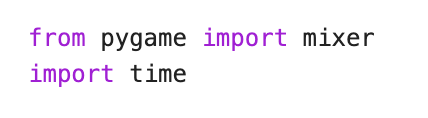
\includegraphics[width=1\linewidth]{template_SGU 2/ImportLibary_Model.png}
\end{center}
\hspace*{0.5cm}Đầu tiên, chúng ta import các thư viện cần thiết: 'pygame', 'time'. Thêm mô-đun mixer từ thư viện pygame cho phép thực hiện các việc đa phương tiên, chẳng hạn như là phát lại âm thanh. Tiếp theo thêm thư viện Time để cho phép kiểm soát thời gian trong chương trình.
\subsubsection{Tạo lớp playlist và playmodel}
\begin{center}
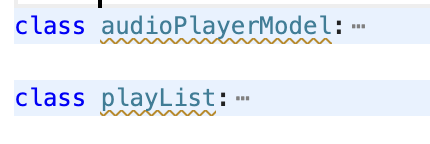
\includegraphics[width=1\linewidth]{template_SGU 2/class_playlist_playmodel.png}
\end{center}
\hspace*{0.5cm} Đầu tiên chúng ta tạo ra lớp phụ playlist đóng vai trò quản lý danh sách phát. Nó chứa các phương thức để chuyển đến bài hát tiếp theo hoặc trước đó trong danh sách phát.

\hspace*{0.5cm} Sau đó chúng ta tạo ra một lớp audioPlayerModel đây là một lớp quan trọng được thiết kế theo mô hình MVC (Model-View-Controller). Mô hình này chứa các phương thức và thuộc tính để điều khiển và quản lý âm nhạc được phát trong ứng dụng.
\subsubsection{Lớp playList}

\begin{center}
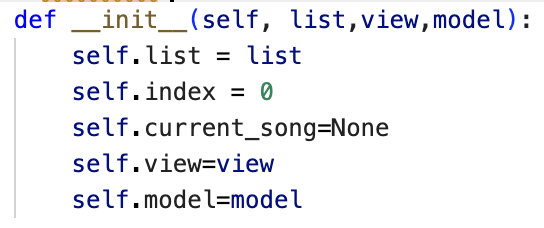
\includegraphics[width=1\linewidth]{template_SGU 2/khoitao_playlist.png}
\end{center}

\hspace*{0.5cm} Đoạn code này khởi tạo phương thức của lớp playList, nhận các tham số là list, view, và model. Các tham số này là danh sách phát, giao diện người dùng và mô hình của ứng dụng.

\begin{center}
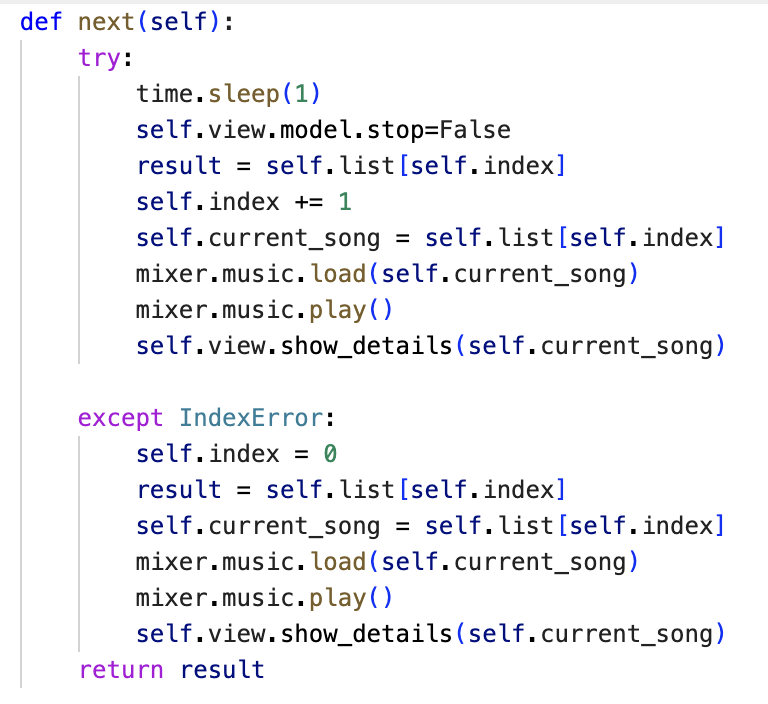
\includegraphics[width=1\linewidth]{template_SGU 2/Playlist_next.png}
\end{center}

\hspace*{0.5cm} Phương thức này cung cấp cơ chế để chuyển đến bài hát tiếp theo trong danh sách phát, xử lý các trường hợp khi đã đến cuối danh sách phát và quay lại phát lại từ đầu nếu cần.

\hspace*{0.5cm} Bắt đầu với một khối lệnh try-except để xử lý ngoại lệ. Dòng time.sleep(1) này tạm ngưng thực thi cho đến khi đã trôi qua 1 giây. Điều này có thể được sử dụng để tạo ra một khoảng thời gian chờ giữa các bài hát. Bắt đầu đặt cờ stop trong mô hình của giao diện người dùng thành False. Điều này có thể được sử dụng để thông báo rằng nhạc đang được phát và không nên dừng lại. Sau đó gán bài hát hiện tại trong danh sách phát vào biến result. self.index += 1 tăng chỉ số của bài hát hiện tại để chuyển đến bài hát tiếp theo trong danh sách phát. Và gán bài hát tiếp theo trong danh sách phát vào biến \texttt{self.current\_song}. Sau đó dùng thư viện mixer tải bài hát tiếp theo trong danh sách phát để chuẩn bị cho việc phát lại. Dùng hàm play() để bắt đầu phát bài hát tiếp theo, cuối cùng hiển thị thông tin chi tiết về bài hát đang được phát lại trên giao diện người dùng. Tương tự như khối lệnh except khi xảy ra lỗi thì ứng dụng sẽ bắt đầu thực hiện phát lại bài hát đầu tiên trong danh sách. Cuối cùng return result trả về bài hát hiện tại để bắt đầu phát lại.

\begin{center}
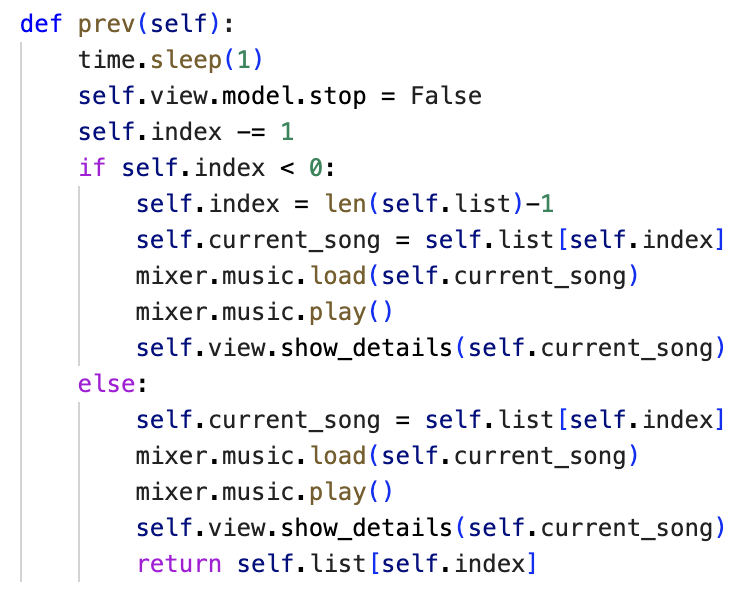
\includegraphics[width=175mm]{template_SGU 2/PlayList_prev.png}
\end{center}

\hspace*{0.5cm} Phương thức này cung cấp cơ chế để chuyển đến bài hát trước đó trong danh sách phát, xử lý trường hợp khi đã ở đầu danh sách phát và quay lại phát lại từ cuối danh sách phát nếu cần.

\hspace*{0.5cm} Thực hiện việc chuyển giao giữa 2 bài hát là 1 giây và đặt cờ hiệu là False. Sau đó giảm chỉ số index - 1  của bài hát hiện tại để chuyển đến bài hát trước trong danh sách phát. Kiểm tra xem chỉ số của bài hát hiện tại đã nhỏ hơn 0 hay chưa. Nếu chỉ số của bài hát hiện tại nhỏ hơn 0, nghĩa là đã đến đầu danh sách phát, ta sẽ đặt chỉ số của bài hát hiện tại là chỉ số của bài hát cuối cùng trong danh sách phát. Sau đó gán bài hát trong danh sách phát vào biến \texttt{self.current\_song}. Và cuối cùng là tải dữ liệu, chạy bài hát và hiển thị thông tin lên giao diện người dùng. Trường hợp nếu chỉ số của bài hát hiện tại không nhỏ hơn 0. Thì gán bài hát trước đó trong danh sách phát vào biến \texttt{self.current\_song} và thực hiện load bài hát, chạy bài hát và hiển thị thông tin lên giao diện người dùng.

\begin{center}
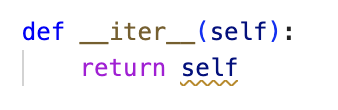
\includegraphics[width=175mm]{template_SGU 2/PlayList_iter.png}
\end{center}

\hspace*{0.5cm} Phương thức này cho phép lớp playList có thể lặp qua các phần tử trong danh sách phát.

\subsubsection{Lớp audioPlayerModel}

\begin{center}
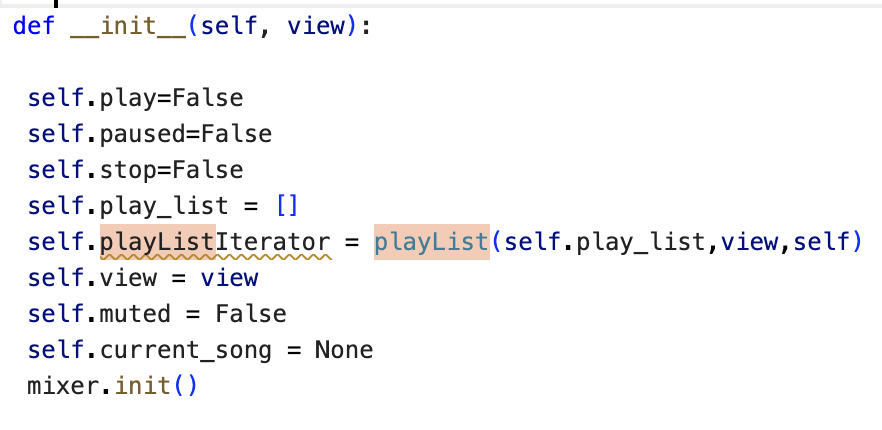
\includegraphics[width=175mm]{template_SGU 2/khoitao_audioPlaymodel.png}
\end{center}

\hspace*{0.5cm} Phương thức khởi tạo này thiết lập các thuộc tính ban đầu của đối tượng audioPlayerModel, bao gồm cài đặt các cờ điều khiển, khởi tạo danh sách phát và các thành phần liên quan đến việc phát lại âm nhạc.

\hspace*{0.5} Đặt biến play thành False, đây là một cờ để xác định xem âm nhạc có đang được phát hay không.

\hspace*{0.5} Đặt biến paused thành False, đây là một cờ để xác định xem âm nhạc có đang được tạm dừng hay không.

\hspace*{0.5} Đặt biến stop thành False, đây là một cờ để xác định xem âm nhạc có đã dừng hay không.

\hspace*{0.5} Khởi tạo danh sách phát rỗng, danh sách này sẽ chứa các bài hát được thêm vào để phát lại.

\hspace*{0.5} \texttt{self.playListIterator = playList(self.play\_list,view,self)}: Khởi tạo một đối tượng của lớp playList, được sử dụng để quản lý việc lặp lại danh sách phát.

\hspace*{0.5} Đặt biến muted thành False, đây là một cờ để xác định xem âm thanh có đang bị tắt hay không.

\hspace*{0.5} Khởi tạo biến \texttt{current\_song} thành None, biến này sẽ chứa thông tin về bài hát hiện đang được phát.

\hspace*{0.5} Khởi tạo mô-đun mixer của pygame để sẵn sàng cho việc phát lại âm thanh.

\begin{center}
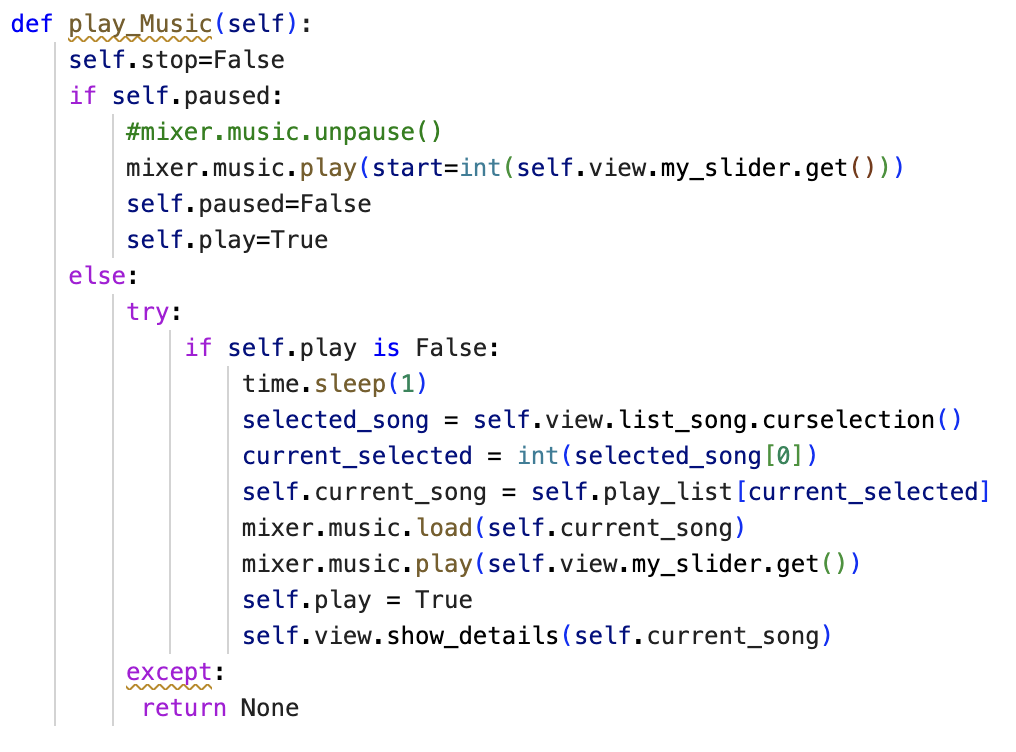
\includegraphics[width=175mm]{template_SGU 2/audio_playMusic.png}
\end{center}

\hspace*{0.5} Phương thức playMusic này cho phép người dùng phát lại âm nhạc từ vị trí đã tạm dừng hoặc phát lại một bài hát mới từ danh sách phát.

\hspace*{0.5} self.stop=False: Đặt biến stop thành False, cho biết rằng âm nhạc chưa được dừng lại.

\hspace*{0.5} Kiểm tra nếu âm nhạc đã được tạm dừng.
\begin{itemize}
    \item mixer.music.play(start=int(self.view.my\_slider.get())): Phát lại âm nhạc từ vị trí được xác định bởi thanh trượt trên giao diện người dùng. Điều này cho phép người dùng tiếp tục phát lại âm nhạc từ vị trí đã tạm dừng trước đó.
    \item self.paused=False: Đặt biến paused thành False, cho biết rằng âm nhạc không còn ở trạng thái tạm dừng nữa.
    \item Và cuối cùng set play=True
\end{itemize}

\hspace*{0.5} Nếu âm nhạc không được tạm dừng trước đó, chúng ta sẽ thực hiện việc phát lại một bài hát mới.
\begin{itemize}
    \item selected\_song = self.view.list\_song.curselection(): Lấy vị trí của bài hát được chọn trong danh sách phát trên giao diện người dùng.
    \item current\_selected = int(selected\_song[0]): Chuyển đổi vị trí được chọn thành một số nguyên.
    \item self.current\_song = self.play\_list[current\_selected]: Gán bài hát được chọn từ danh sách phát vào biến current\_song.
    \item Tải bài hát được chọn và chuẩn bị cho việc bắt đầu phát lại. Hiển thị thông tin chi tiết lên giao diện.
\end{itemize}

\hspace*{0.5} Xử lý ngoại lệ nếu có bất kỳ lỗi nào xảy ra trong quá trình phát lại âm nhạc. return None: Trả về None nếu có lỗi xảy ra trong quá trình phát lại âm nhạc.

\begin{center}
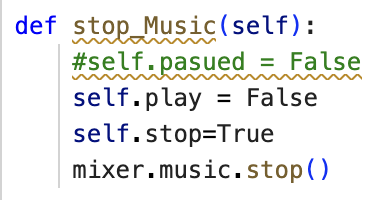
\includegraphics[width=175mm]{template_SGU 2/audio_stop.png}
\end{center}

\hspace*{0.5} Phương thức này cung cấp một cách an toàn để dừng phát âm nhạc và cập nhật trạng thái của các biến điều khiển trong lớp audioPlayerModel.

\begin{itemize}
    \item self.play = False: Đặt biến play thành False, cho biết rằng không có bài hát nào đang được phát hiện tại.
    \item self.stop=True: Đặt biến stop thành True, cho biết rằng âm nhạc đã được dừng lại.
    \item mixer.music.stop(): Dừng phát lại âm nhạc bằng cách gọi phương thức stop() từ mô-đun mixer của pygame.
\end{itemize}

\begin{center}
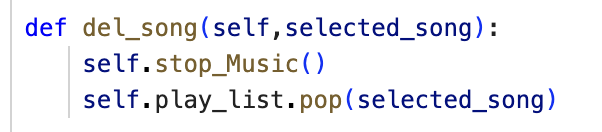
\includegraphics[width=175mm]{template_SGU 2/audio_delsong.png}
\end{center}

\hspace*{0.5} Phương thức này kết hợp việc dừng phát âm nhạc và xóa bài hát khỏi danh sách phát một cách an toàn, giúp đảm bảo rằng việc xóa bài hát không gây ra vấn đề gì đối với hoạt động của ứng dụng.

\begin{itemize}
    \item self.stop\_Music(): Gọi phương thức stop\_Music() để dừng phát lại âm nhạc. Điều này đảm bảo rằng âm nhạc sẽ dừng lại trước khi bài hát được xóa khỏi danh sách phát.
    \item self.play\_list.pop(selected\_song): Xóa bài hát được chỉ định khỏi danh sách phát. Phương thức pop() loại bỏ phần tử tại vị trí chỉ định (selected\_song) khỏi danh sách và trả về giá trị của phần tử đó.
\end{itemize}

\begin{center}
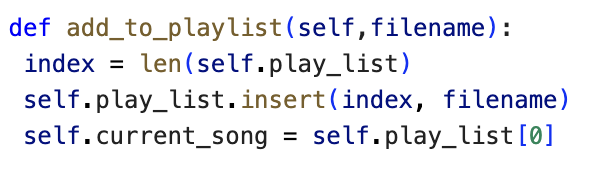
\includegraphics[width=175mm]{template_SGU 2/audio_addto.png}
\end{center}

\hspace*{0.5} Phương thức này cho phép thêm một bài hát vào danh sách phát và cập nhật bài hát hiện đang được chọn để phát lại nếu không có bài hát nào khác đang phát.

\begin{itemize}
    \item index = len(self.play\_list): Tính độ dài hiện tại của danh sách phát để xác định vị trí mới của bài hát sẽ được thêm vào.
    \item self.play\_list.insert(index, filename): Chèn bài hát được chỉ định (filename) vào danh sách phát tại vị trí cuối cùng của danh sách.
    \item self.current\_song = self.play\_list[0]: Gán bài hát đầu tiên trong danh sách phát vào biến current\_song, đảm bảo rằng bài hát mới thêm vào sẽ được chọn để phát lại nếu không có bài hát nào khác đang được phát.
\end{itemize}

\begin{center}
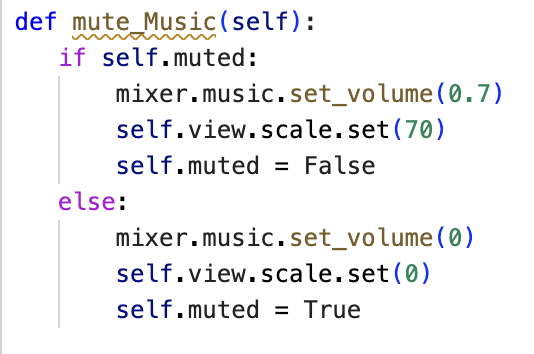
\includegraphics[width=175mm]{template_SGU 2/audio_mute.png}
\end{center}

\hspace*{0.5} Phương thức này cho phép người dùng tắt hoặc bật âm thanh của âm nhạc và cập nhật trạng thái hiển thị trên giao diện người dùng tương ứng.

\begin{itemize}
    \item Kiểm tra biến mute nếu ở trạng thái true thì âm thanh sẽ bị tắt bằng cách set\_volume = 0.
    \item Còn nếu kiểm tra biến mute ở trạng thái false thì âm thanh sẽ được điều chỉnh mặc định ở mức 70\%.
\end{itemize}

\begin{center}
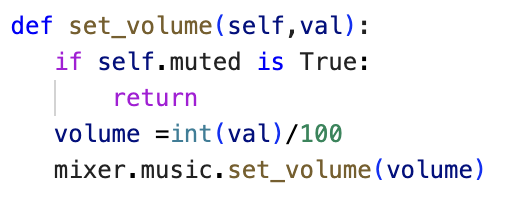
\includegraphics[width=175mm]{template_SGU 2/audio_volume.png}
\end{center}

\hspace*{0.5} Phương thức này cho phép cài đặt âm lượng của âm nhạc dựa trên giá trị được chỉ định và kiểm tra xem âm thanh có đang bị tắt hay không trước khi thực hiện thay đổi.

\begin{itemize}
    \item if self.muted is True:: Kiểm tra xem âm thanh có đang bị tắt hay không.
    \item Nếu âm thanh đã bị tắt (self.muted==True), phương thức sẽ kết thúc mà không làm gì cả, do không cần thiết phải thay đổi âm lượng khi âm thanh đã được tắt.
    \item Nếu âm thanh không bị tắt tạo biến volume=int(val)/100: Chuyển đổi giá trị của val từ định dạng phần trăm sang giá trị thực của âm lượng (từ 0 đến 1).
    \item mixer.music.set\_volume(volume): Đặt âm lượng của âm nhạc thành giá trị volume đã tính toán.
\end{itemize}

\begin{center}
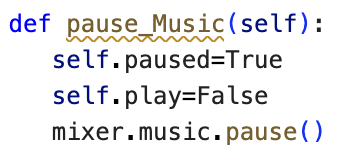
\includegraphics[width=175mm]{template_SGU 2/audio_pause.png}
\end{center}

\hspace*{0.5} Phương thức này cho phép tạm dừng âm nhạc và cập nhật trạng thái của các biến điều khiển trong lớp audioPlayerModel tương ứng.

\begin{itemize}
    \item self.paused=True: Đặt biến paused thành True, cho biết rằng âm nhạc đang ở trạng thái tạm dừng.
    \item self.play=False: Đặt biến play thành False, cho biết rằng không có bài hát nào đang được phát lại.
    \item mixer.music.pause(): Tạm dừng phát lại âm nhạc bằng cách gọi phương thức pause() từ mô-đun mixer của pygame.
\end{itemize}

\begin{center}
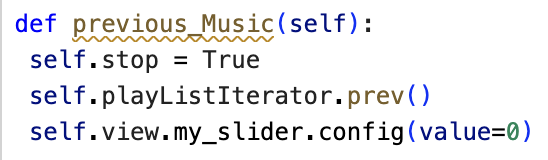
\includegraphics[width=175mm]{template_SGU 2/audio_previous.png}
\end{center}

\hspace*{0.5} Phương thức này cung cấp khả năng chuyển đến bài hát trước đó trong danh sách phát và cập nhật trạng thái của thanh trượt trên giao diện người dùng.

\begin{itemize}
    \item self.stop = True: Đặt biến stop thành True, cho biết rằng việc chuyển đến bài hát trước đó đang được thực hiện.
    \item self.playListIterator.prev(): Gọi phương thức prev() từ đối tượng playListIterator để di chuyển đến bài hát trước đó trong danh sách phát.
    \item self.view.my\_slider.config(value=0): Thiết lập giá trị của thanh trượt trên giao diện người dùng về 0, đảm bảo rằng thanh trượt sẽ được đặt lại khi chuyển đến bài hát trước đó.
\end{itemize}

\begin{center}
\includegraphics[width=175mm]{template_SGU 2/audio_next.png}
\end{center}

\hspace*{0.5} Phương thức này cung cấp khả năng chuyển đến bài hát tiếp theo trong danh sách phát và cập nhật trạng thái của thanh trượt trên giao diện người dùng.

\begin{itemize}
    \item Đặt biến stop thành True cho biết việc dừng bài hát và cbi cho việc chuyển đến bài hát tiếp theo.
    \item Gọi phương thức next() từ đối tượng playListIterator để di chuyển đến bài hát tiếp theo trong danh sách phát.
    \item Thiết lập giá trị của thanh trượt trên giao diện người dùng về 0, đảm bảo rằng thanh trượt sẽ được đặt lại khi chuyển đến bài hát tiếp theo.
\end{itemize}

\begin{center}
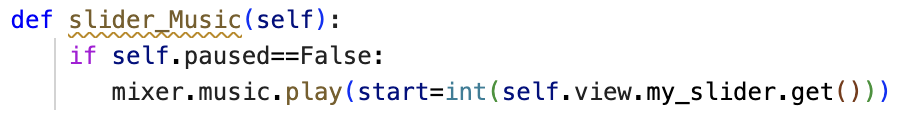
\includegraphics[width=175mm]{template_SGU 2/audio_slider.png}
\end{center}

\hspace*{0.5} Phương thức này cho phép điều chỉnh vị trí phát lại của âm nhạc dựa trên vị trí hiện tại của thanh trượt trên giao diện người dùng và đảm bảo rằng âm nhạc sẽ tiếp tục phát lại từ vị trí mới được chọn.

\begin{itemize}
    \item if self.paused==False: Kiểm tra xem âm nhạc có đang trong trạng thái không bị tạm dừng hay không.
    \item mixer.music.play(start=int(self.view.my\_slider.get())): Nếu âm nhạc không bị tạm dừng, phương thức sẽ phát lại âm nhạc từ vị trí được xác định bởi giá trị hiện tại của thanh trượt trên giao diện người dùng. Điều này cho phép người dùng chuyển đến một vị trí cụ thể trong bài hát bằng cách di chuyển thanh trượt.
\end{itemize}

\begin{center}
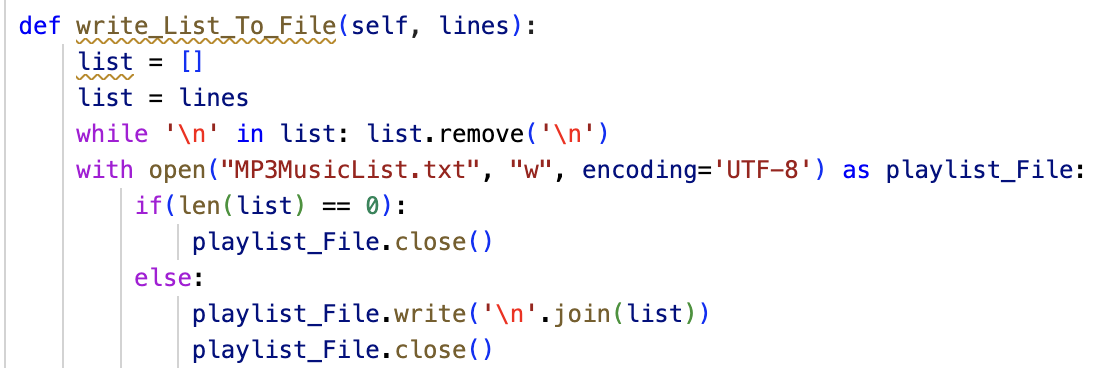
\includegraphics[width=175mm]{template_SGU 2/audio_write_List.png}
\end{center}

\hspace*{0.5} Phương thức này cho phép ghi danh sách các bài hát vào một tệp văn bản với mã hóa UTF-8, loại bỏ các ký tự xuống dòng không mong muốn, và đảm bảo rằng tệp văn bản được đóng sau khi hoàn tất việc ghi.

\begin{itemize}
    \item Bắt đầu khởi tạo một danh sách tróng list=[].
    \item Gán danh sách đầu vào (lines) cho danh sách mới được khởi tạo. Điều này sẽ sao chép tất cả các phần tử từ danh sách đầu vào sang danh sách mới.
    \item while '\n' in list: list.remove('\n'): Loại bỏ các ký tự xuống dòng ('\n') khỏi danh sách mới. Điều này đảm bảo rằng danh sách sẽ không chứa bất kỳ ký tự xuống dòng nào.
    \item with open("MP3MusicList.txt", "w", encoding='UTF-8') as playlist\_File: Mở tệp văn bản có tên "MP3MusicList.txt" để ghi dữ liệu. Tệp này sẽ được mở trong chế độ ghi ("w"), có mã hóa UTF-8.
    \item Kiểm tra xem danh sách có rỗng hay không. Nếu rỗng thì hoàn tất việc ghi file.
    \item Nếu danh sách không rỗng thì thực hiện các việc sau: playlist\_File.write('\n'.join(list)): Ghi nội dung của danh sách vào tệp văn bản, mỗi phần tử trên một dòng. Phương thức join() được sử dụng để nối các phần tử trong danh sách với ký tự xuống dòng ('\n') giữa chúng. Sau đó hoàn tất việc ghi file và kết thúc file.
\end{itemize}

\subsection{Xây dựng PlayerView}
\subsubsection{Import thư viện}

\begin{center}
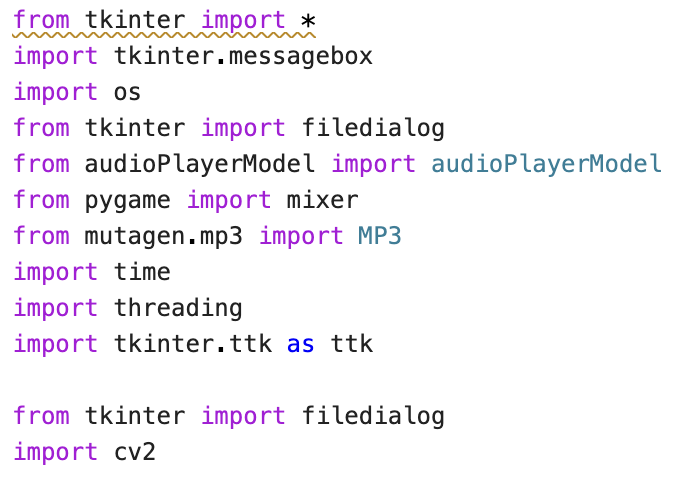
\includegraphics[width=135mm]{template_SGU 2/importlibary_View.png}
\end{center}

\hspace*{0.5} Đầu tiên, chúng ta import các thư viện cần thiết như: 'tkinter', 'os', 'pygame.mixer', 'mutagen.mp3', 'time', 'threading', 'cv2' và trình xử lý logic từ model audioPlayerModel. Thư viện tkinter được sử dụng để tạo giao diện người dùng đồ họa trong Python, os cho phép tương tác với hệ thống tập tin, pygame.mixer được sử dụng để phát âm thanh, mutagen.mp3 được sử dụng để độc thông tin từ các tệp MP3, time được xử dụng để quản lý thời gian, threading cho phép thực các  tác vụ đồng thời, cv2 thư viện OpenCV cho phép làm việc với video ,và audioPlayerModel sử dụng logic để quản lý việc phát lại âm nhạc và tương tác với người dùng thông qua giao diện người dùng.

\subsubsection{Khởi tạo lớp audioPlayerView}
\begin{center}
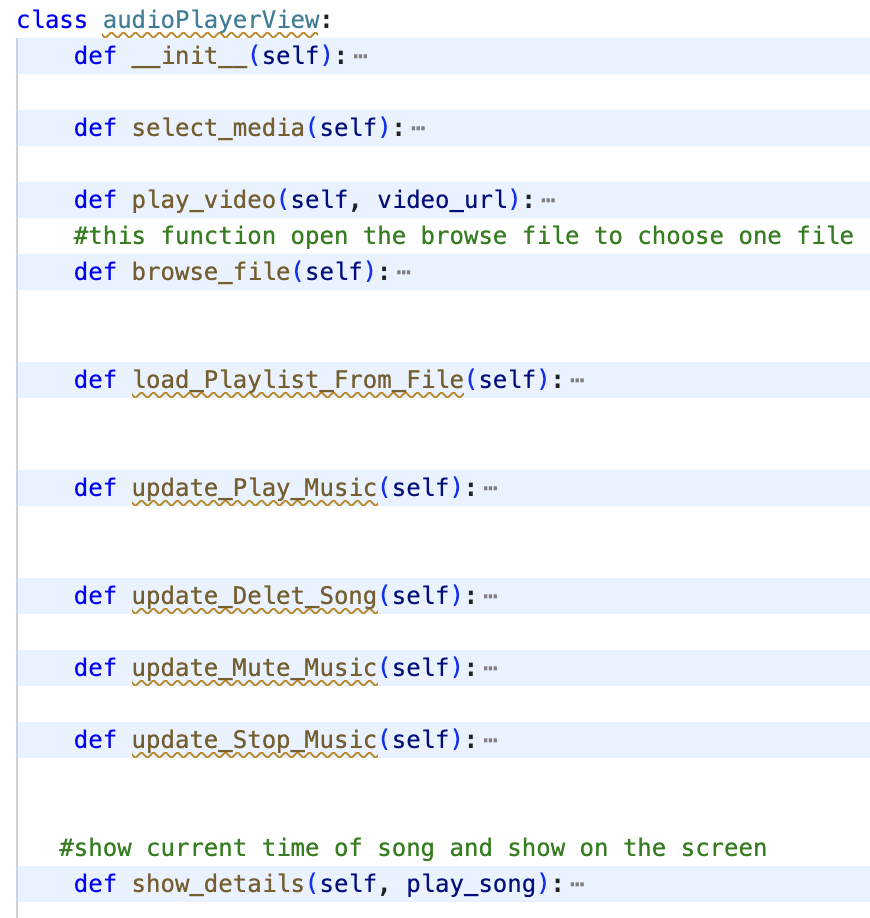
\includegraphics[width=80mm]{template_SGU 2/khoitao_View1.png}
\end{center}
\begin{center}
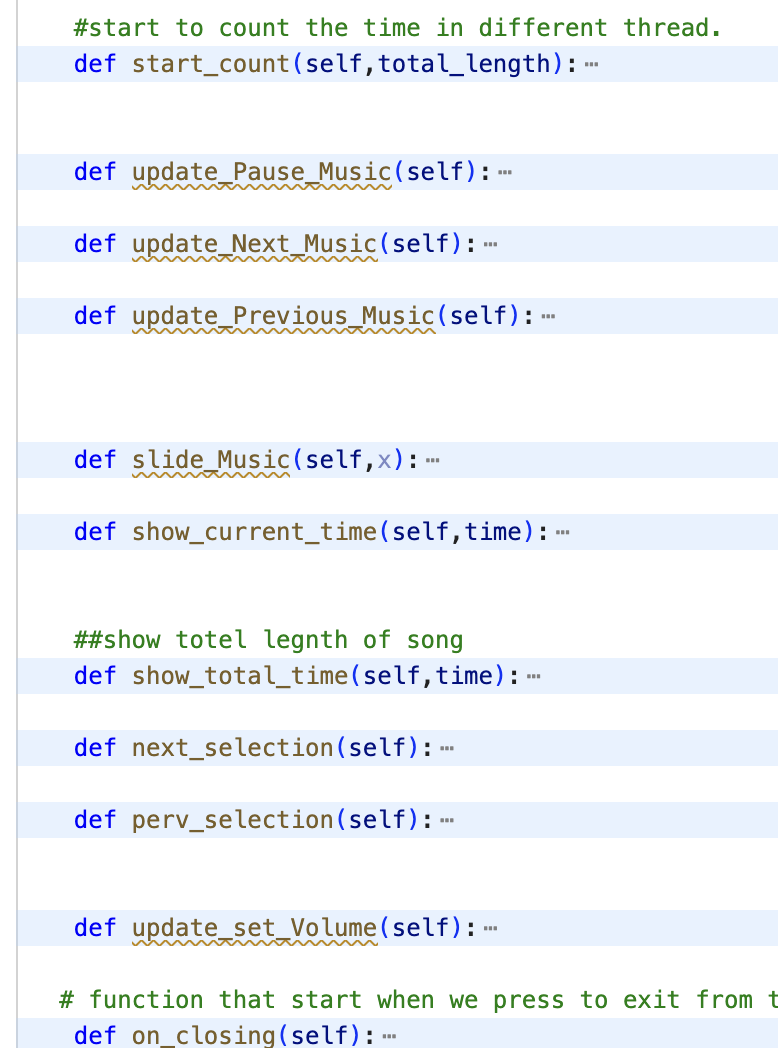
\includegraphics[width=80mm]{template_SGU 2/khoitao_View2.png}
\end{center}
\begin{itemize}
    \item \_\_init\_\_(): Khởi tạo giao diện người dùng, các thành phần UI như nút, thanh trượt, hộp danh sách và hộp thoại.
    \item Các phương thức update\_*\_Music(): Được gọi khi người dùng tương tác với các nút như Play, Pause, Stop, Next, Previous để điều khiển phát lại âm nhạc.
    \item Các phương thức browse\_file(), load\_Playlist\_From\_File(): Được sử dụng để tải danh sách bài hát từ một tệp văn bản và cho phép người dùng chọn bài hát từ hệ thống tệp.
    \item Các phương thức show\_current\_time(), show\_total\_time(): Được sử dụng để hiển thị thời gian hiện tại và tổng thời gian của bài hát đang được phát lại.
    \item Phương thức start\_count(): Sử dụng để tính thời gian hiện tại của bài hát và cập nhật thanh trượt thời gian của bài hát.
    \item Phương thức on\_closing(): Được gọi khi ứng dụng đóng, để lưu danh sách bài hát hiện tại vào một tệp văn bản trước khi thoát.
    \item Phương thức select\_media() và play\_video(): Cho phép người dùng chọn và phát video bằng cách sử dụng thư viện OpenCV.
\end{itemize}
\subsubsection{Các phương thức được khởi tạo}
\begin{center}
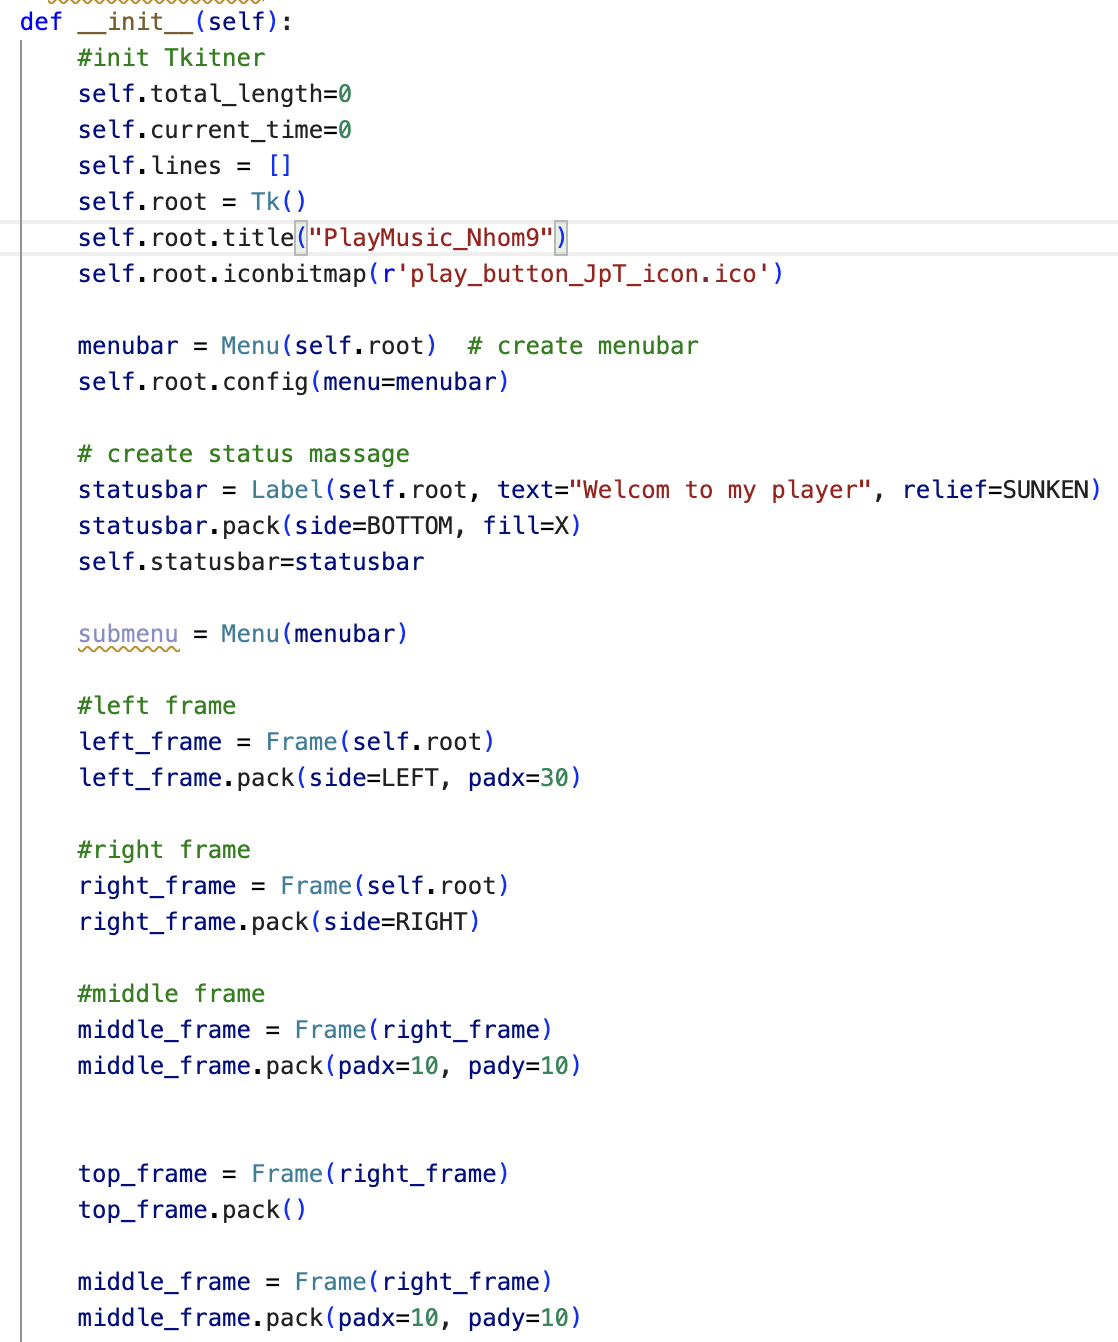
\includegraphics[width=80mm]{template_SGU 2/view_init_1.png}
\end{center}
\begin{center}
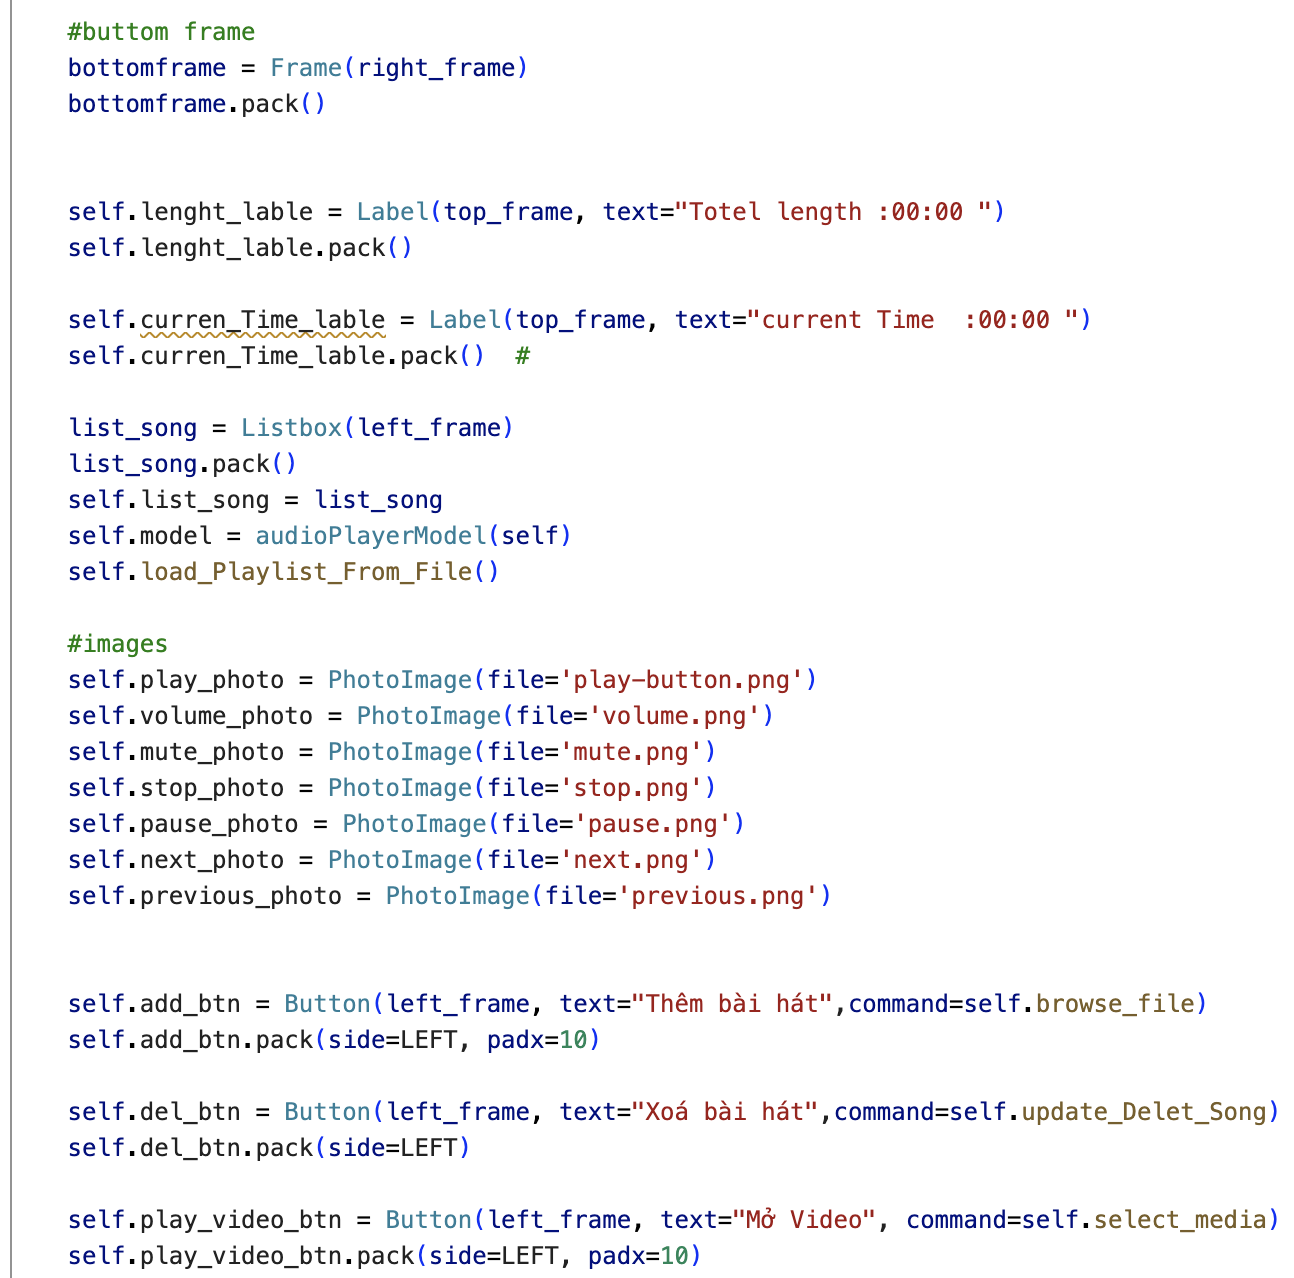
\includegraphics[width=80mm]{template_SGU 2/view_init_2.png}
\end{center}
\begin{center}
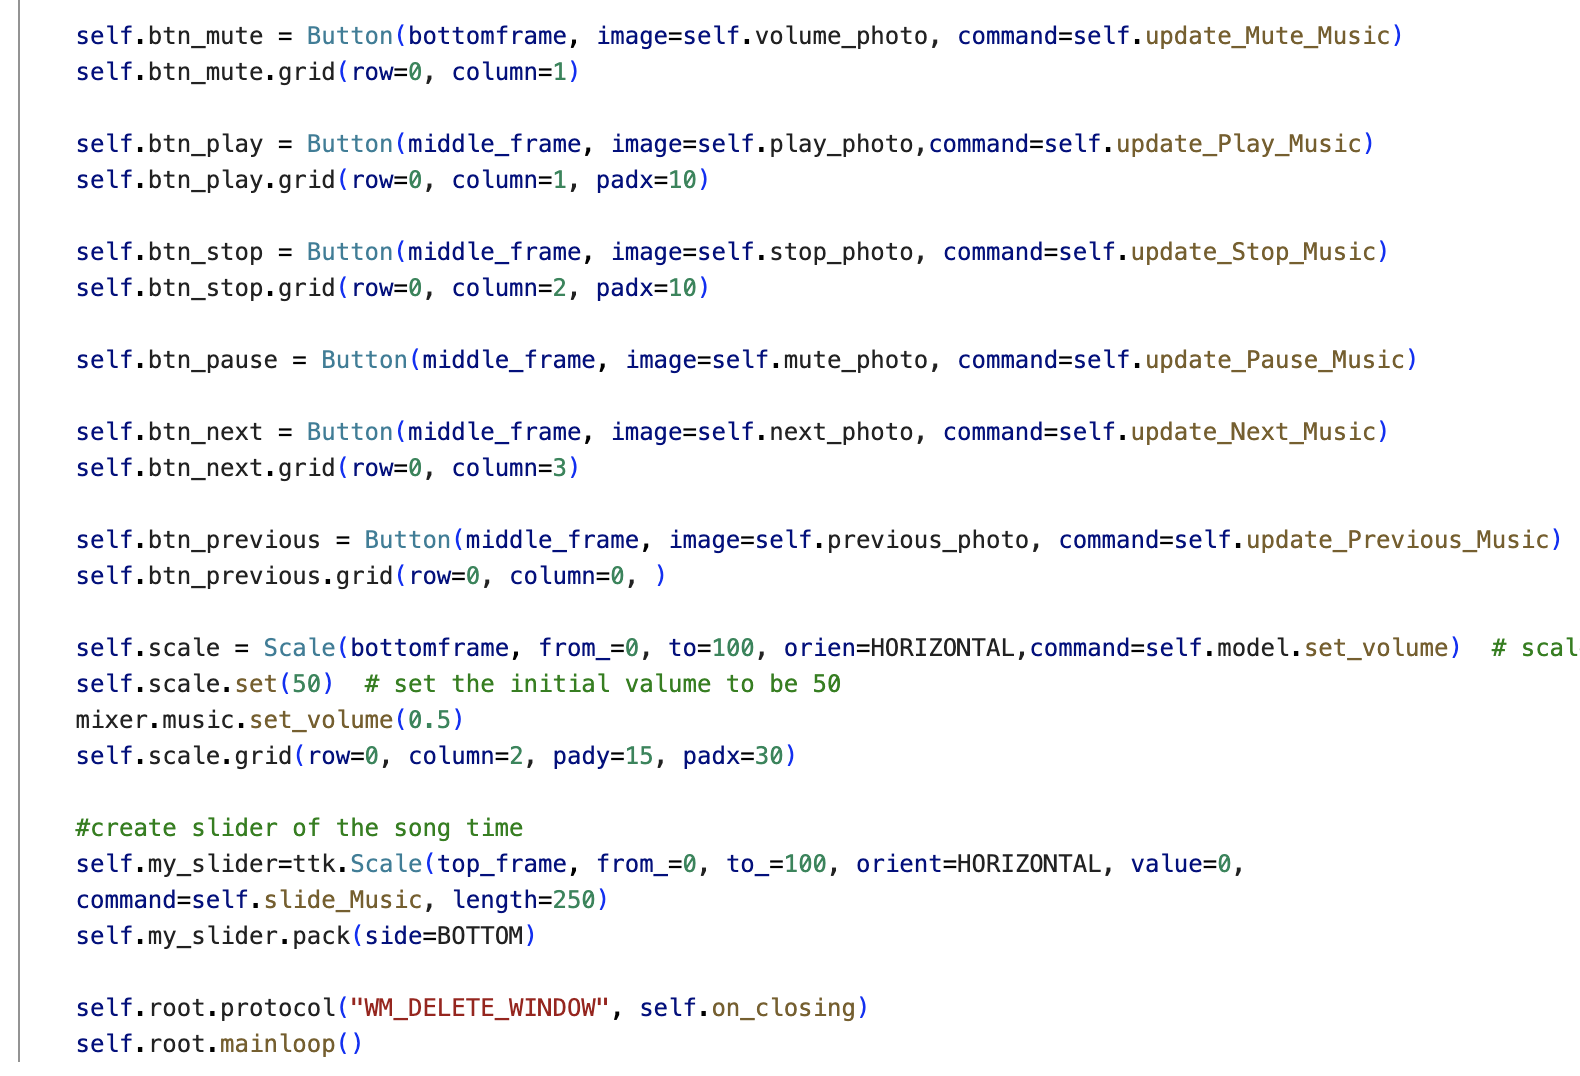
\includegraphics[width=80mm]{template_SGU 2/view_init_3.png}
\end{center}
\hspace*{0.5} Phương thức \_\_init\_\_() này cung cấp cấu trúc cơ bản cho giao diện người dùng của ứng dụng và kết nối các hành động của người dùng với các chức năng xử lý của ứng dụng.

\begin{itemize}
    \item Khởi tạo cửa sổ giao diện: Một cửa sổ Tkinter được tạo ra với tiêu đề "PlayMusic\_Nhom9" và biểu tượng (icon) được thiết lập bằng hình ảnh play\_button\_JpT\_icon.ico. Một thanh trạng thái (status bar) được tạo để hiển thị các thông điệp "Welcom to my player" và được đặt ở phía dưới cùng của cửa sổ.
    \item Tạo khung và các thành phần giao diện: Các khung (frames) được tạo ra để sắp xếp các thành phần của giao diện người dùng. Các thành phần như nhãn (label), danh sách (listbox), và các nút (button) được thêm vào các khung tương ứng.
    \item Tải danh sách bài hát từ tệp và khởi tạo các hình ảnh: Danh sách bài hát được tải từ tệp MP3MusicList.txt và hiển thị trong hộp danh sách. Các hình ảnh (biểu tượng) được tải từ các tệp hình ảnh để sử dụng cho các nút như Play, Pause, Stop, và các nút khác.
    \item Gắn các hàm xử lý sự kiện với các nút: Để thực hiện các hành động như thêm bài hát, xóa bài hát, mở video, điều khiển phát lại âm nhạc, vv.
    \item Tạo thanh trượt và thực hiện sự kiện đóng cửa sổ: Thanh trượt được tạo để điều chỉnh âm lượng và thời gian của bài hát. Sự kiện đóng cửa sổ được gắn với phương thức on\_closing() để lưu danh sách bài hát vào tệp trước khi ứng dụng đóng.
\end{itemize}

\begin{center}
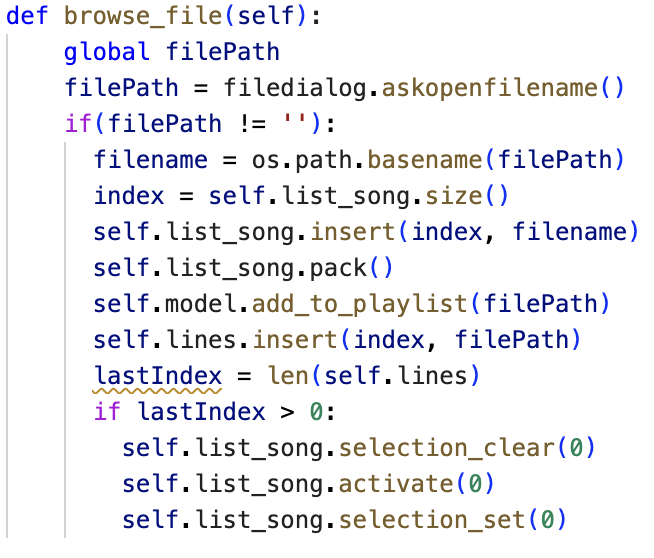
\includegraphics[width=80mm]{template_SGU 2/view_browse.png}
\end{center}
\hspace*{0.5} Phương thức browse\_file(self) được sử dụng để mở hộp thoại chọn tệp và thêm tệp được chọn vào danh sách bài hát của ứng dụng.
\begin{itemize}
    \item Đầu tiên dùng filedialog.askopenfilename(): Để mở hộp thoại chọn tệp và trả về đường dẫn của tệp đã chọn.
    \item Sau đó kiểm tra xem đã chọn tệp hay chưa. Nếu đã chọn tệp thì lấy tên tệp từ đường dẫn đã được chọn, sau đó lấy số lượng mục hiện có trong danh sách bài hát, bắt đầu thêm tên tệp vào danh sách bài hát ở vị trí cuối cùng. Sau đó cập nhật và hiển thị danh sách bài hát, dùng model.add\_to\_playlist để lưu đường dẫn của tệp vào danh sách phát trong mô hình, kế tiếp là thêm đường dẫn của tệp vào danh sách đường dẫn trong giao diện người dùng. Cuối cùng là lấy độ dài của danh sách đường dẫn.
    \item Nếu như độ dài của danh sách đường dẫn có ít nhất 1 phần tử thì bỏ chọn tất cả các mục trong danh sách sau đó kích hoạt và chọn mục đầu tiên trong danh sách phát, .
\end{itemize}

\begin{center}
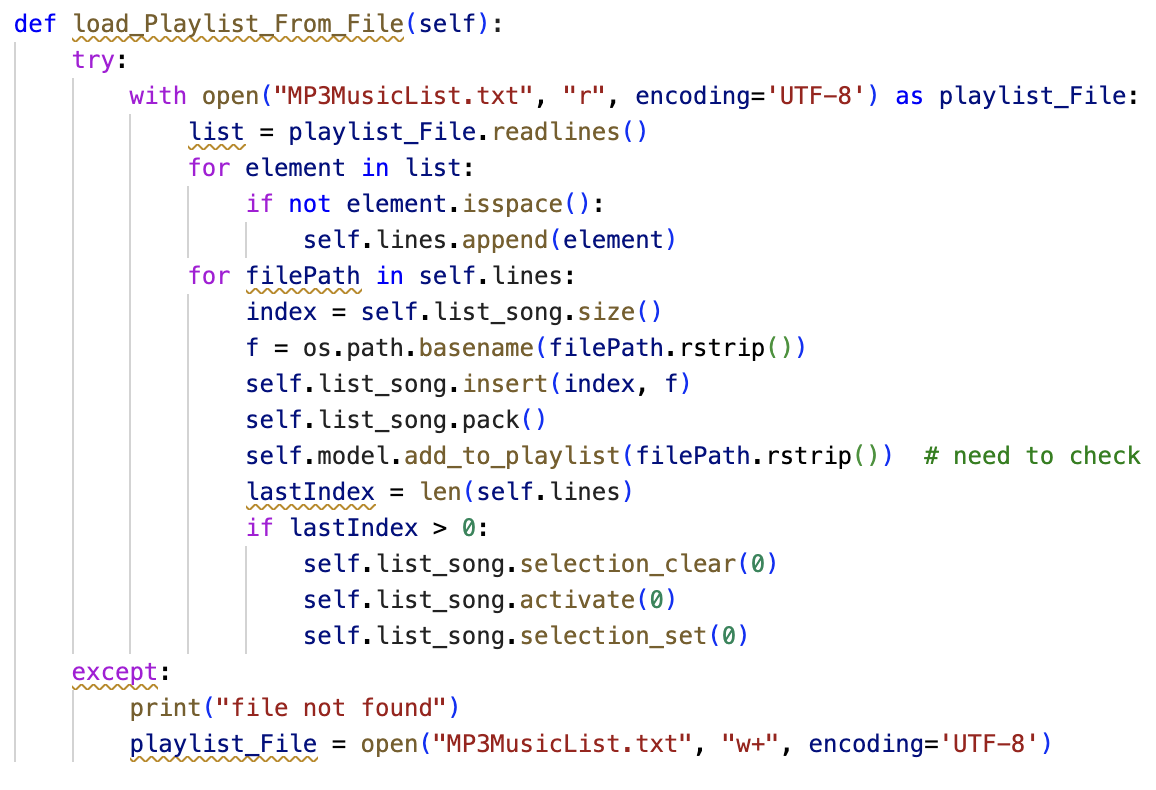
\includegraphics[width=80mm]{template_SGU 2/audio_loadPlay.png}
\end{center}
\hspace*{0.5} Phương thức load\_Playlist\_From\_File(self) được sử dụng để đọc danh sách các bài hát từ tệp "MP3MusicList.txt" và hiển thị chúng trong giao diện người dùng. Thêm đường dẫn của các bài hát vào danh sách phát trong mô hình người dùng. Hiển thị tên của các bài hát trong danh sách bên trong giao diện người dùng. Khi người dùng khởi chạy ứng dụng, phương thức này được gọi để tải danh sách các bài hát đã lưu trước đó từ tệp "MP3MusicList.txt" vào giao diện người dùng.
\begin{itemize}
    \item Đầu tiên chúng ta mở tệp MP3MusicList.txt để đọc nội dung bằng cách sử dụng câu lệnh with nhầm đảm bảo khi không còn sử dụng thì tệp sẽ được tự động đống.
    \item Dùng hàm readlines() để đọc nội dung của tệp và lưu vào danh sách list, trong đó mỗi dòng của tệp là một phần tử trong danh sách.
    \item Dùng hàm for để duyệt qua từng phần tử của danh sách list và bắt đầu kiểm tra từng phần tử đó có phải là khoảng trắng hết hay không. Nếu là khoảng trắng hết thì nó không được thêm vào danh sách.
    \item Tiếp theo duyệt qua từng phần tử trong danh sách bài hát, và lấy tên đường dẫn lưu vào biến f, sau đó thêm tên tệp vào danh sách phát của người dùng và thêm đường dẫn vào danh sách phát của mô hình người dùng.
\end{itemize}

\begin{center}
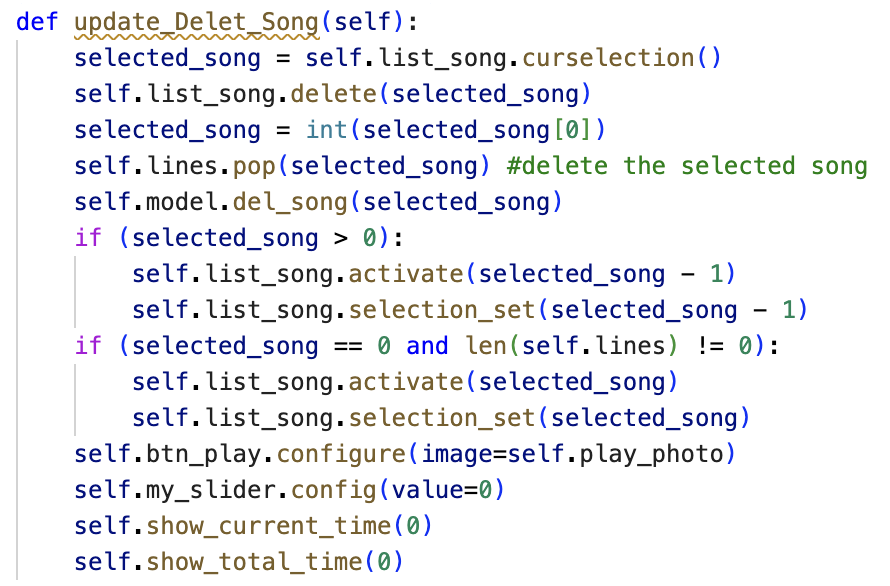
\includegraphics[width=130mm]{template_SGU 2/audio_updateDelet.png}
\end{center}
\begin{itemize}
    \item Phương thức này được gọi khi người dùng muốn xóa một bài hát khỏi danh sách phát.
    \item Đầu tiên, nó lấy ra bài hát được chọn bằng cách sử dụng phương thức curselection() của đối tượng Listbox list\_song.
    \item Sau đó, nó xóa bài hát được chọn từ danh sách bằng cách sử dụng phương thức delete() của Listbox.
    \item Tiếp theo, nó loại bỏ bài hát đã chọn khỏi danh sách bằng cách sử dụng phương thức pop() trên danh sách lines.
    \item Sau khi xóa, nó gọi phương thức del\_song() của đối tượng model để xóa bài hát khỏi danh sách phát trong model.
    \item Nếu bài hát được xóa không phải là bài hát cuối cùng trong danh sách, nó chọn bài hát tiếp theo trong danh sách bằng cách thay đổi chỉ mục được kích hoạt và chỉ mục được chọn trong Listbox.
    \item Nếu bài hát được xóa là bài hát đầu tiên trong danh sách và danh sách không trống, nó cũng chọn bài hát tiếp theo trong danh sách.
    \item Cuối cùng, nó cập nhật hình ảnh của nút play sang hình ảnh ban đầu (play\_photo), thiết lập giá trị của thanh trượt của slider về 0, và cập nhật hiển thị thời gian hiện tại và thời gian tổng cộng của bài hát sang giá trị mặc định là 0.
\end{itemize}

\begin{center}
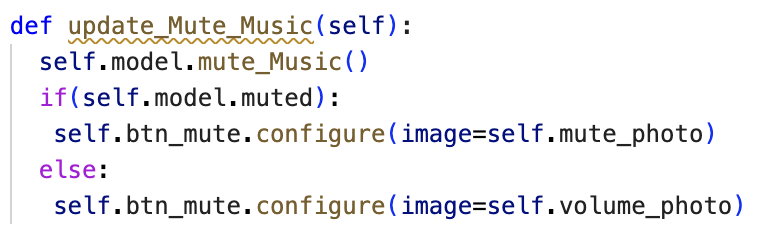
\includegraphics[width=130mm]{template_SGU 2/audio_updateMute.png}
\end{center}
\begin{itemize}
    \item Phương thức này được gọi khi người dùng muốn tắt hoặc bật âm thanh.
    \item Đầu tiên, nó gọi phương thức mute\_Music() của đối tượng model để tắt hoặc bật âm thanh.
    \item Nếu âm thanh đã được tắt, nó cập nhật hình ảnh của nút mute sang hình ảnh mute (mute\_photo). Nếu âm thanh được bật, nó cập nhật hình ảnh của nút mute sang hình ảnh volume (volume\_photo). Điều này giúp người dùng biết trạng thái hiện tại của âm thanh.
\end{itemize}

\begin{center}
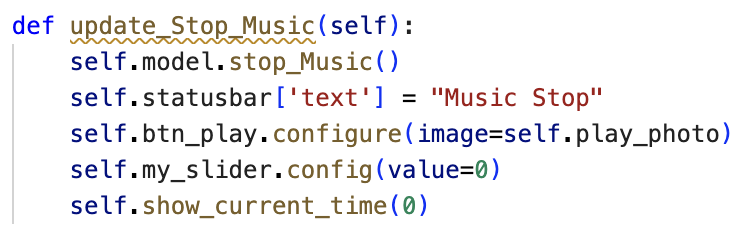
\includegraphics[width=130mm]{template_SGU 2/audio_updateStop.png}
\end{center}
\begin{itemize}
    \item Phương thức này được gọi khi người dùng muốn tắt bài hát.
    \item Đầu tiên, nó gọi phương thức stop\_Music() của đối tượng model để dừng nhạc.
    \item Sau đó, nó cập nhật văn bản của thanh trạng thái (statusbar) để thông báo rằng âm nhạc đã dừng.
    \item Tiếp theo, nút phát nhạc (btn\_play) được cấu hình để hiển thị hình ảnh của nút phát (play\_photo), để người dùng biết rằng âm nhạc có thể được phát lại từ đầu.
    \item Thanhs trượt thời gian của bài hát (my\_slider) được cài đặt lại về giá trị ban đầu là 0.
    \item Cuối cùng, thời gian hiện tại của bài hát (current\_time) được cập nhật và hiển thị trên giao diện người dùng bằng cách gọi phương thức show\_current\_time(0) với tham số là 0, tức là thời gian bắt đầu.
\end{itemize}

\begin{center}
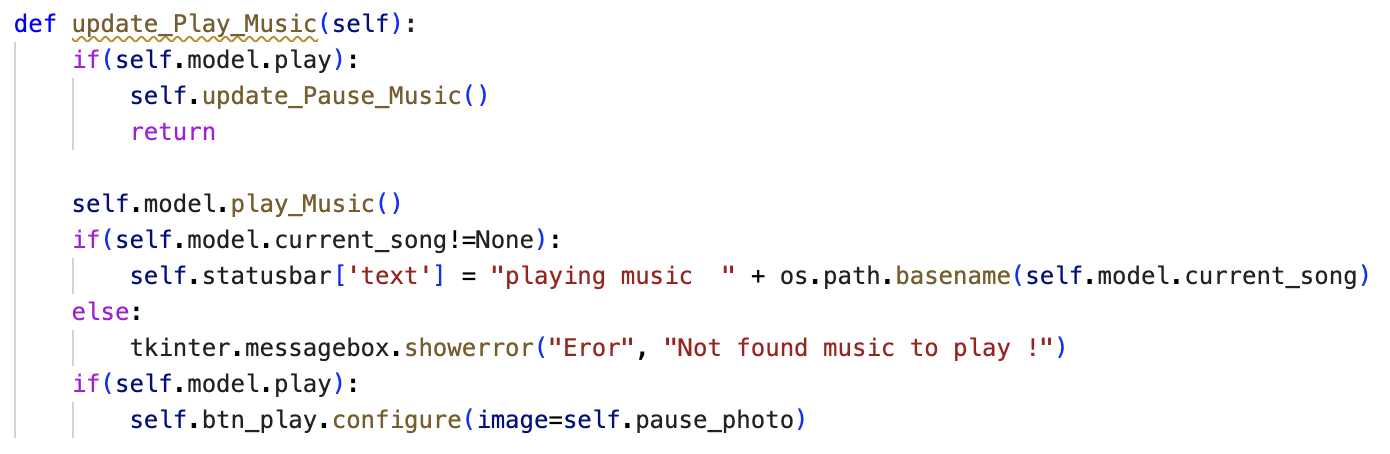
\includegraphics[width=130mm]{template_SGU 2/audio_updatePlay.png}
\end{center}
\begin{itemize}
    \item Phương thức này kiểm tra xem có đang phát nhạc không bằng cách kiểm tra giá trị của biến play trong đối tượng model. Nếu đang phát, nó gọi phương thức update\_Pause\_Music để tạm dừng nhạc và trả về ngay sau đó.
    \item Nếu không đang phát nhạc, nó gọi phương thức play\_Music của đối tượng model để bắt đầu phát nhạc. Nếu bài hát hiện tại không tồn tại, nó hiển thị một hộp thoại thông báo lỗi. Nếu bắt đầu phát nhạc thành công, nó cập nhật thanh trạng thái để hiển thị tên của bài hát đang phát và thay đổi hình ảnh của nút play sang hình ảnh tạm dừng (pause\_photo).
\end{itemize}

\begin{center}
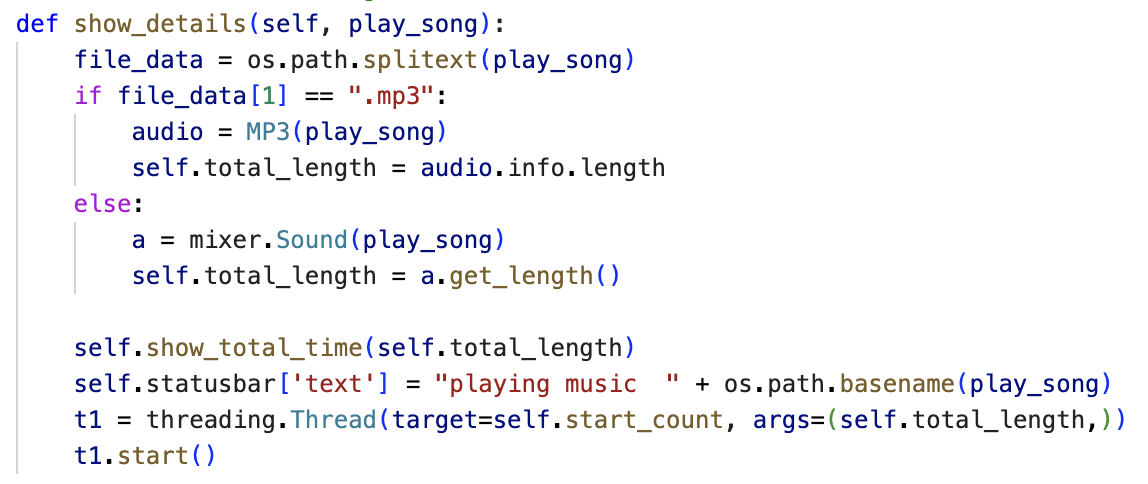
\includegraphics[width=130mm]{template_SGU 2/audio_showdetail.png}
\end{center}
\begin{itemize}
    \item Phương thức này được sử dụng để hiển thị chi tiết về bài hát đang được phát, bao gồm độ dài tổng cộng của bài hát và tên bài hát trên thanh trạng thái.
    \item Đầu tiên, phương thức này nhận đầu vào là đường dẫn của bài hát đang được phát (play\_song).
    \item Tiếp theo, nó kiểm tra phần mở rộng của tệp âm thanh (play\_song). Nếu nó là một tệp MP3, nó sẽ sử dụng thư viện Mutagen để lấy thông tin về độ dài của bài hát bằng cách tạo một đối tượng MP3 và truy cập thuộc tính info.length. Nếu không, nó sẽ sử dụng thư viện Pygame để lấy độ dài của bài hát bằng cách tạo một đối tượng mixer.Sound và gọi phương thức get\_length().
    \item Sau đó, nó gọi phương thức show\_total\_time để hiển thị độ dài tổng cộng của bài hát trên giao diện người dùng.
    \item Tiếp theo, nó cập nhật văn bản của thanh trạng thái để hiển thị tên của bài hát đang được phát
    \item Cuối cùng, nó tạo một luồng mới (threading.Thread) để bắt đầu đếm thời gian của bài hát bằng cách gọi phương thức start\_count với tham số là độ dài tổng cộng của bài hát.
\end{itemize}

\begin{center}
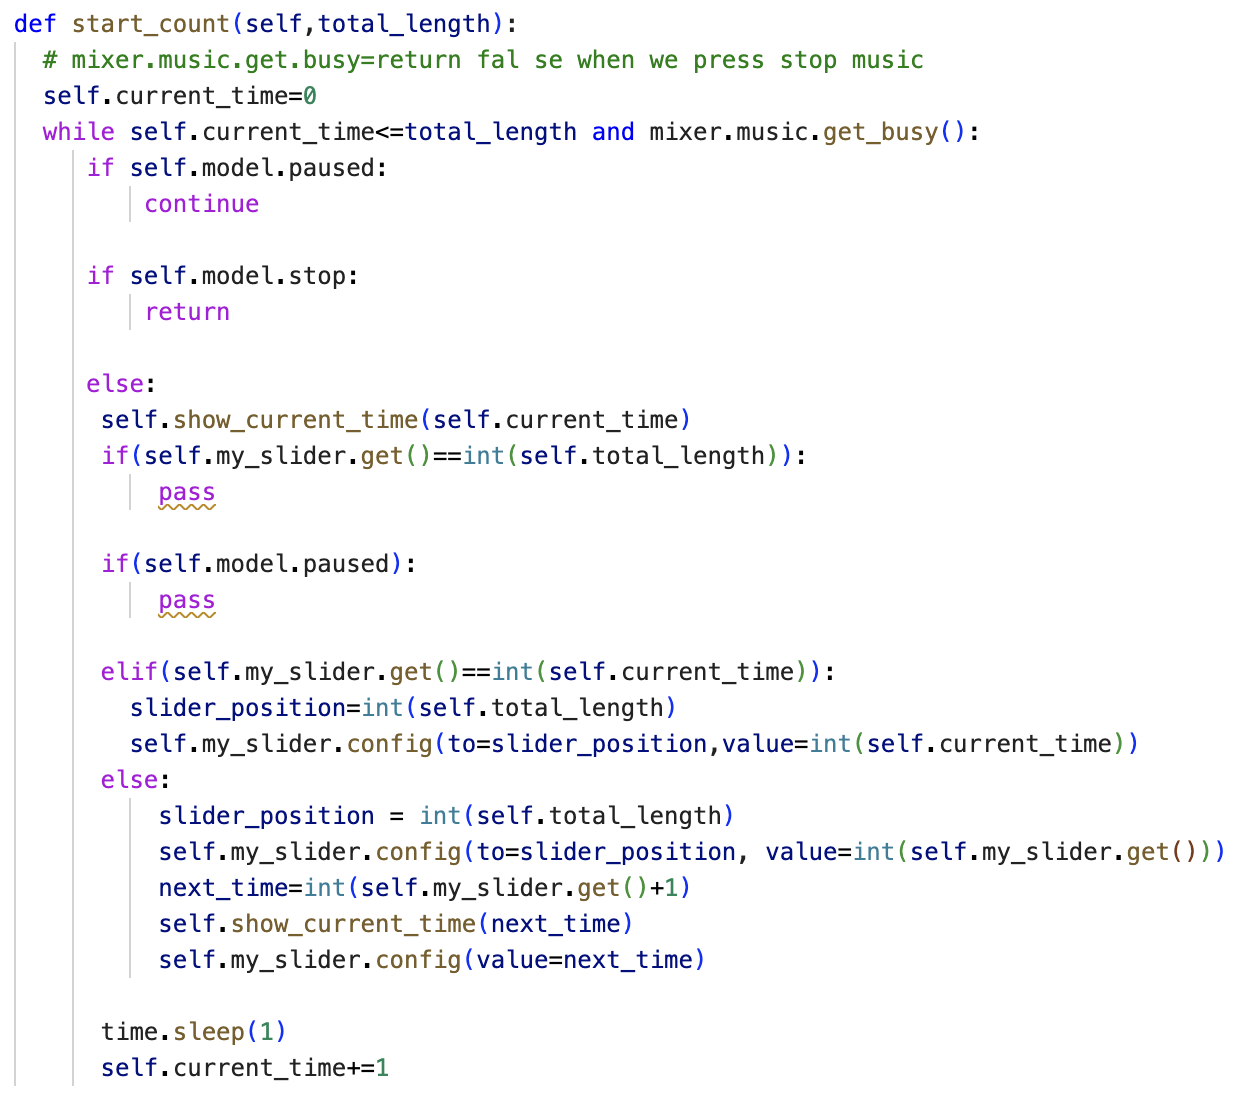
\includegraphics[width=130mm]{template_SGU 2/audio_start_count.png}
\end{center}
\begin{itemize}
    \item Phương thức này được sử dụng để bắt đầu đếm thời gian của bài hát đang phát và cập nhật thanh trượt thời gian của bài hát trên giao diện người dùng.
    \item Đầu tiên, nó khởi tạo biến self.current\_time để đếm thời gian hiện tại của bài hát.
    \item Tiếp theo, nó sử dụng một vòng lặp while để tiếp tục đếm thời gian cho đến khi thời gian hiện tại vượt quá độ dài tổng cộng của bài hát hoặc khi âm nhạc dừng lại.
    \item Trong vòng lặp, nếu âm nhạc đang tạm dừng (self.model.paused là True), vòng lặp sẽ tiếp tục mà không làm gì cả.
    \item Nếu âm nhạc được dừng (self.model.stop là True), vòng lặp sẽ kết thúc.
    \item Nếu không, nó cập nhật thời gian hiện tại của bài hát trên giao diện người dùng bằng cách gọi phương thức show\_current\_time.
    \item Nếu thanh trượt thời gian của bài hát đã đạt đến cuối cùng, không làm gì cả.
    \item Nếu không, nếu thanh trượt thời gian hiện tại của bài hát trên giao diện người dùng bằng với thời gian hiện tại (self.my\_slider.get() là int(self.current\_time)), thanh trượt sẽ được cập nhật để di chuyển đến cuối cùng của bài hát.
    \item Nếu không, nó sẽ cập nhật vị trí của thanh trượt để di chuyển theo thời gian hiện tại của bài hát.
    \item Cuối cùng, sau mỗi giây, nó tăng thời gian hiện tại lên 1 giây và chờ một giây trước khi tiếp tục vòng lặp.
\end{itemize}

\begin{center}
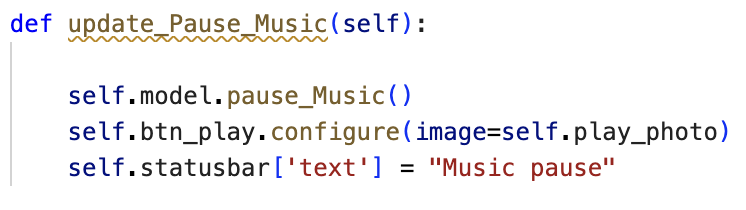
\includegraphics[width=130mm]{template_SGU 2/audio_updatePause.png}
\end{center}
\begin{itemize}
    \item Phương thức này được sử dụng để tạm dừng hoặc tiếp tục phát nhạc khi người dùng nhấn vào nút phát/pause trên giao diện người dùng.
    \item Đầu tiên, nó gọi phương thức pause\_Music từ đối tượng self.model, điều này sẽ tạm dừng hoặc tiếp tục phát nhạc, tùy thuộc vào trạng thái hiện tại của âm nhạc.
    \item Sau đó, nó cập nhật hình ảnh của nút phát/pause để hiển thị hình ảnh phù hợp. Nếu âm nhạc được tạm dừng, nút sẽ chuyển sang hình ảnh phát; nếu âm nhạc đang phát, nút sẽ chuyển sang hình ảnh tạm dừng.
    \item Cuối cùng, nó cập nhật thanh trạng thái (statusbar) trên giao diện người dùng để hiển thị thông báo "Music pause".
\end{itemize}

\begin{center}
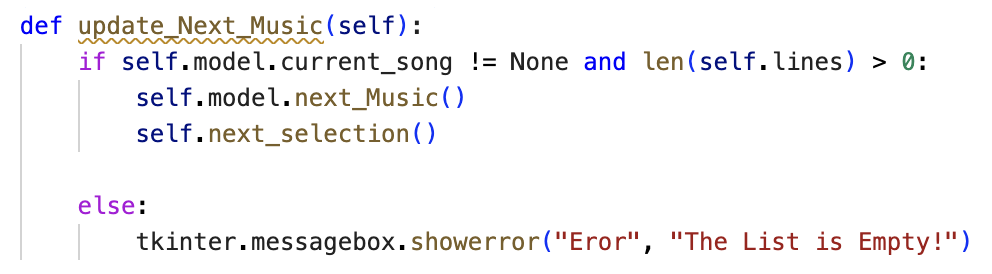
\includegraphics[width=130mm]{template_SGU 2/audio_updateNext.png}
\end{center}
\begin{itemize}
    \item Phương thức này được sử dụng để chuyển đến bài hát kế tiếp trong danh sách phát khi người dùng nhấn vào nút "Next".
    \item Đầu tiên, nó kiểm tra xem có bài hát đang được phát và danh sách phát có ít nhất một bài hát không. Nếu cả hai điều kiện này đều đúng, nó tiến hành chuyển đến bài hát tiếp theo bằng cách gọi phương thức next\_Music từ đối tượng self.model.
    \item Sau đó, nó gọi phương thức next\_selection để cập nhật việc chọn bài hát tiếp theo trong danh sách phát trên giao diện người dùng.
    \item Nếu không có bài hát nào đang được phát hoặc danh sách phát trống, nó hiển thị một thông báo lỗi sử dụng tkinter.messagebox.showerror.
\end{itemize}

\begin{center}
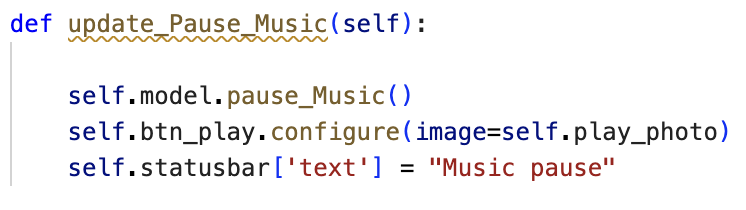
\includegraphics[width=130mm]{template_SGU 2/audio_updatePause.png}
\end{center}
\begin{itemize}
    \item Phương thức này được sử dụng để chuyển đến bài hát trước đó trong danh sách phát khi người dùng nhấn vào nút "Previous".
    \item Đầu tiên, nó kiểm tra xem có bài hát đang được phát và danh sách phát có ít nhất một bài hát không. Nếu cả hai điều kiện này đều đúng, nó tiến hành chuyển đến bài hát trước đó bằng cách gọi phương thức previous\_Music từ đối tượng self.model.
    \item Sau đó, nó gọi phương thức perv\_selection để cập nhật việc chọn bài hát trước đó trong danh sách phát trên giao diện người dùng.
    \item Nếu không có bài hát nào đang được phát hoặc danh sách phát trống, nó hiển thị một thông báo lỗi sử dụng tkinter.messagebox.showerror.
\end{itemize}

\begin{center}
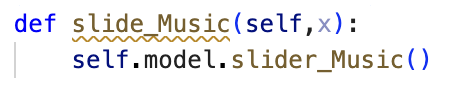
\includegraphics[width=130mm]{template_SGU 2/audio_slide.png}
\end{center}
\begin{itemize}
    \item Phương thức slide\_Music trong lớp audioPlayerView được gọi khi trượt thanh trượt của bài hát trên thanh trượt thời gian. Khi người dùng thay đổi vị trí của thanh trượt, giá trị mới của thanh trượt được chuyển đến phương thức slider\_Music trong đối tượng self.model, để điều chỉnh thời gian phát của bài hát tương ứng. Điều này giúp người dùng có thể tua nhanh chóng đến một phần của bài hát mà họ muốn nghe.
\end{itemize}

\begin{center}
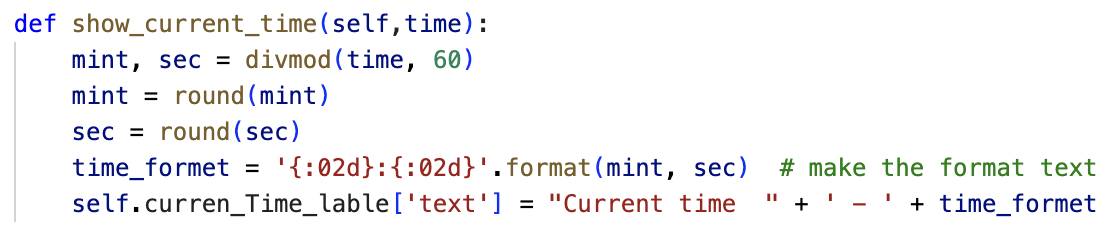
\includegraphics[width=130mm]{template_SGU 2/audio_showCurrentTime.png}
\end{center}
\begin{itemize}
    \item Phương thức show\_current\_time trong lớp audioPlayerView nhận đầu vào là time, đại diện cho thời gian hiện tại của bài hát được phát, tính bằng giây. Phương thức này chuyển đổi thời gian từ định dạng giây thành định dạng phút và giây, sau đó cập nhật nhãn hiển thị thời gian hiện tại trên giao diện người dùng. Định dạng hiển thị của thời gian là hai chữ số cho phút và giây, được hiển thị trong nhãn curren\_Time\_lable.
\end{itemize}

\begin{center}
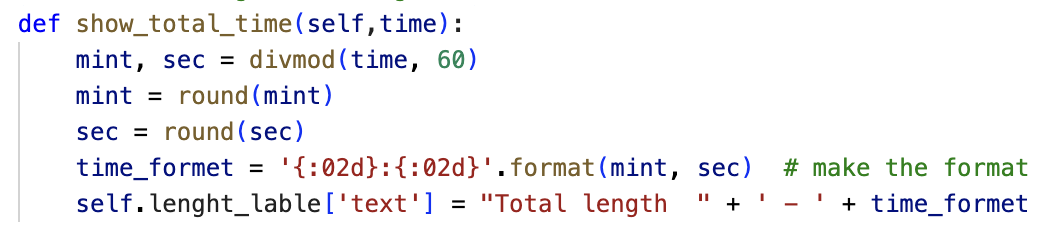
\includegraphics[width=130mm]{template_SGU 2/audio_showTotalTime.png}
\end{center}
\begin{itemize}
    \item Phương thức show\_total\_time trong lớp audioPlayerView nhận đầu vào là time, đại diện cho tổng thời lượng của bài hát được phát, tính bằng giây. Phương thức này chuyển đổi thời gian từ định dạng giây thành định dạng phút và giây, sau đó cập nhật nhãn hiển thị tổng thời lượng trên giao diện người dùng. Định dạng hiển thị của thời lượng là hai chữ số cho phút và giây, được hiển thị trong nhãn lenght\_lable.
\end{itemize}

\begin{center}
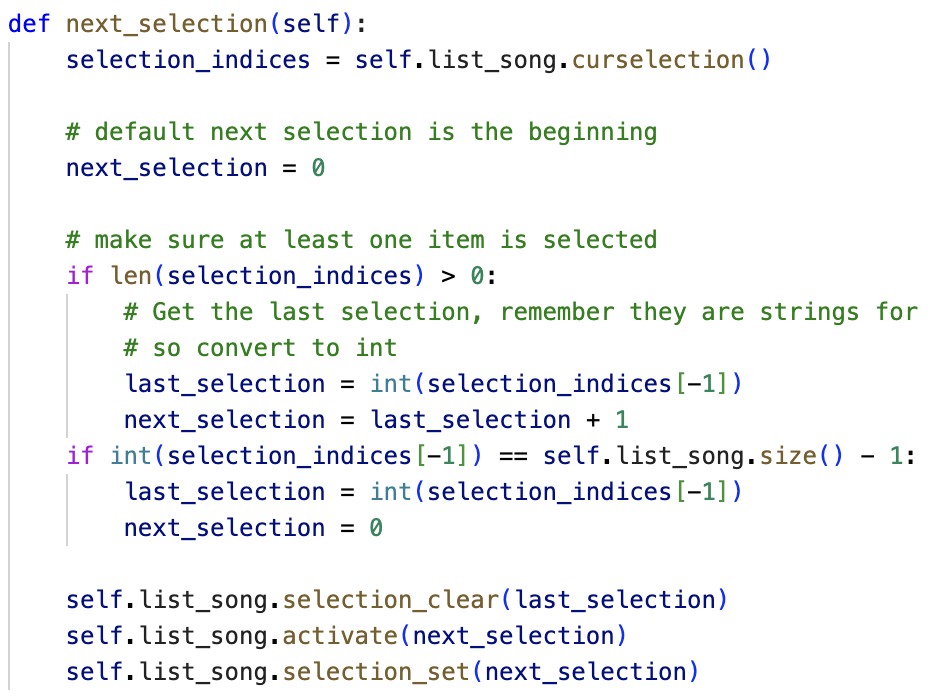
\includegraphics[width=130mm]{template_SGU 2/audio_Next.png}
\end{center}
\begin{itemize}
    \item Phương thức next\_selection trong lớp audioPlayerView được sử dụng để chọn bài hát tiếp theo trong danh sách phát khi người dùng nhấn nút "Next". Phương thức này thực hiện các bước sau:
    \item Lấy chỉ số của các bài hát đang được chọn trong danh sách.
    \item Nếu có ít nhất một mục được chọn, phương thức tính toán chỉ số của bài hát tiếp theo dựa trên bài hát cuối cùng được chọn.
    \item Nếu bài hát cuối cùng được chọn là bài hát cuối cùng trong danh sách, phương thức chọn bài hát đầu tiên làm bài hát tiếp theo.
    \item Dọn dẹp lựa chọn trước đó, kích hoạt bài hát tiếp theo và đặt lựa chọn cho bài hát đó.
\end{itemize}

\begin{center}
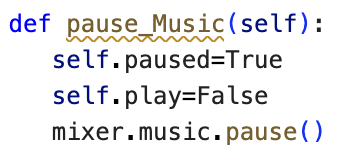
\includegraphics[width=130mm]{template_SGU 2/audio_pause.png}
\end{center}
\begin{itemize}
    \item Phương thức perv\_selection trong lớp audioPlayerView thực hiện chức năng chọn bài hát trước đó trong danh sách phát khi người dùng nhấn nút "Previous". Phương thức này thực hiện các bước sau:
    \item Lấy chỉ số của các bài hát đang được chọn trong danh sách.
    \item Xác định chỉ số của bài hát trước đó dựa trên bài hát cuối cùng được chọn.
    \item Nếu bài hát cuối cùng được chọn là bài hát đầu tiên trong danh sách, phương thức chọn bài hát cuối cùng làm bài hát trước đó.
    \item Dọn dẹp lựa chọn trước đó, kích hoạt bài hát trước đó và đặt lựa chọn cho bài hát đó.
\end{itemize}

\begin{center}
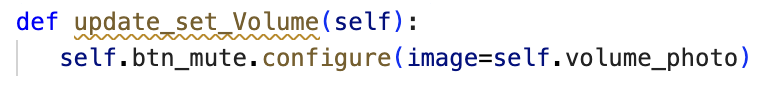
\includegraphics[width=130mm]{template_SGU 2/audio_updatesetVolume.png}
\end{center}
\begin{itemize}
    \item Phương thức update\_set\_Volume trong lớp audioPlayerView thực hiện chức năng update lại hình ảnh của nút tắt âm thanh khi người dùng giảm âm lượng xuống mức 0.
\end{itemize}

\begin{center}
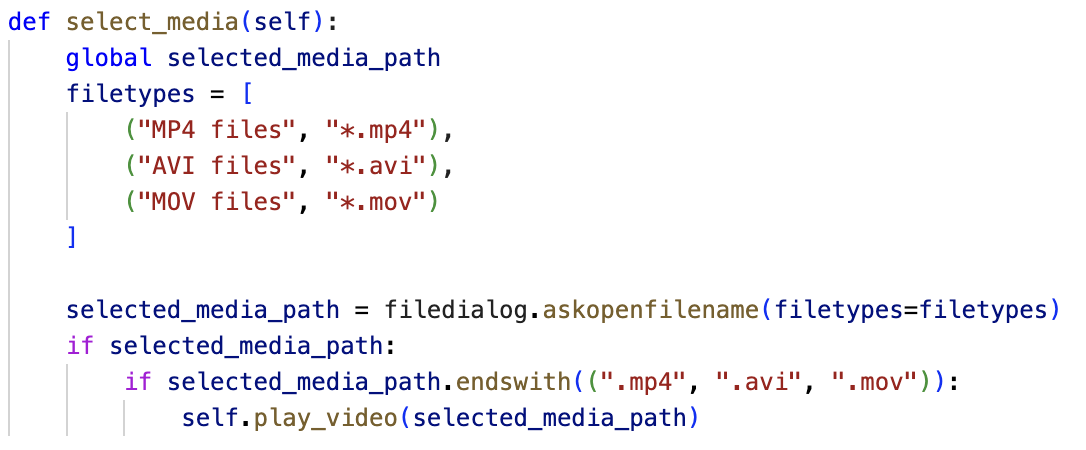
\includegraphics[width=130mm]{template_SGU 2/audio_select_media.png}
\end{center}
\begin{itemize}
    \item Phương thức select\_media trong lớp audioPlayerView thực hiện nhiệm vụ cho phép người dùng chọn một tệp phương tiện (video) từ hộp thoại mở tệp và sau đó chạy video nếu tệp đó hợp lệ.
    \item Khởi tạo biến toàn cục selected\_media\_path: Biến này được sử dụng để lưu đường dẫn đến tệp phương tiện được chọn bởi người dùng. Việc sử dụng biến toàn cục cho phép hàm này và các phương thức khác có thể truy cập đến đường dẫn tệp được chọn.
    \item Định dạng các loại tệp: Trước hết, hàm xác định loại các tệp mà người dùng có thể chọn bằng cách định nghĩa danh sách các loại tệp và các mẫu tìm kiếm tương ứng (ví dụ: MP4, AVI, MOV).
    \item Hiển thị hộp thoại mở tệp: Hàm askopenfilename từ thư viện filedialog được sử dụng để hiển thị hộp thoại mở tệp cho người dùng. Hộp thoại này sẽ hiển thị các tệp phương tiện dựa trên các loại tệp đã được định nghĩa trước đó.
    \item Xác định loại tệp được chọn: Sau khi người dùng chọn một tệp, hàm kiểm tra xem tệp đó có phải là một tệp video hợp lệ hay không bằng cách kiểm tra phần mở rộng của tên tệp.
    \item Chạy video nếu tệp hợp lệ: Nếu tệp được chọn là một tệp video hợp lệ (có phần mở rộng là .mp4, .avi, hoặc .mov), hàm sẽ gọi phương thức play\_video với đường dẫn của tệp video làm đối số.
    
\end{itemize}

\begin{center}
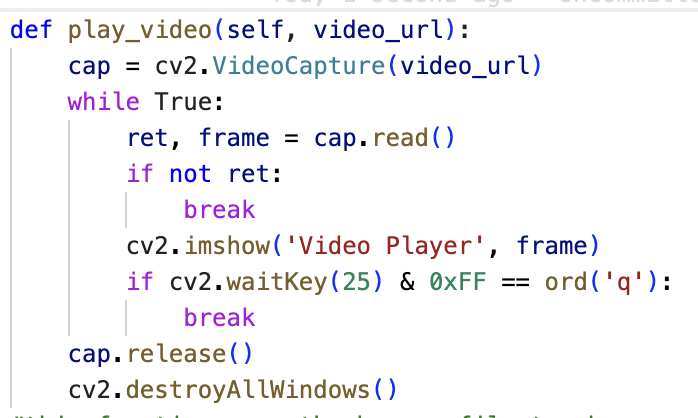
\includegraphics[width=130mm]{template_SGU 2/audio_playVideo.png}
\end{center}
\begin{itemize}
    \item Phương thức select\_media trong lớp audioPlayerView thực hiện nhiệm vụ phát video từ một tệp video có đường dẫn được chỉ định.
    \item Mở tệp video: Hàm sử dụng phương thức cv2.VideoCapture từ thư viện OpenCV để mở tệp video. Đường dẫn của tệp video được truyền vào qua tham số video\_url.
    \item Vòng lặp phát video: Hàm bắt đầu một vòng lặp vô hạn để đọc từng khung hình từ video một cách tuần tự. Trong mỗi lần lặp, hàm sử dụng phương thức cap.read() để đọc một khung hình mới từ video.
    \item Hiển thị khung hình: Sau khi một khung hình mới được đọc từ video, hàm sử dụng phương thức cv2.imshow để hiển thị khung hình đó trên một cửa sổ mới có tên là "Video Player".
    \item Thoát khỏi vòng lặp: Vòng lặp sẽ tiếp tục cho đến khi hết video hoặc người dùng nhấn phím 'q' trên bàn phím. Khi điều kiện này xảy ra, vòng lặp sẽ dừng và các cửa sổ hiển thị video sẽ đóng.
    \item Giải phóng tài nguyên: Sau khi kết thúc vòng lặp, hàm giải phóng tài nguyên bằng cách gọi phương thức cap.release() để đóng tệp video và cv2.destroyAllWindows() để đóng tất cả các cửa sổ hiển thị video.
    
\end{itemize}

\begin{center}
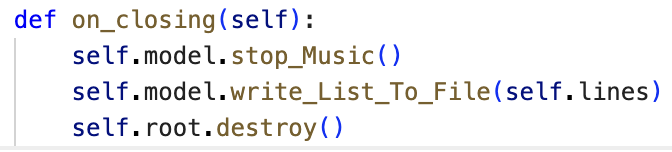
\includegraphics[width=130mm]{template_SGU 2/audio_onClosing.png}
\end{center}
\begin{itemize}
    \item Phương thức on\_closing trong lớp audioPlayerView là một hàm được gọi khi người dùng đóng ứng dụng. Chức năng chính của nó là dừng phát nhạc, sau đó lưu danh sách những bài hát hiện tại vào tệp tin và cuối cùng là đóng ứng dụng.
\end{itemize}

\section{Cài đặt vày chạy ứng dụng}
\hspace*{0.5cm} Đối với nhà phát triển:

\hspace*{0.5cm}Trước khi chạy ứng dụng, đảm bảo bạn đã cài đặt các phụ thuộc sau:
\begin{itemize}
    \item Python 3.x
    \item Tkinter
    \item Pygame
    \item OS
    \item Mutagen
    \item Time
    \item Threading
    \item OpenCV
\end{itemize}

Bạn có thể cài đặt các thư viện phụ thuộc bằng pip:

\hspace*{0.5cm} pip3 install pygame

\hspace*{0.5cm} pip3 install mutagen

\hspace*{0.5cm} pip3 install opencv-python-headless


Cách sử dụng:

\hspace*{0.5cm} Clone the Repository:\href{https://github.com/hung573/PlayAudio_PlayVideo} {https://github.com/hung573/PlayAudio_PlayVideo}

\hspace*{1cm} git clone https://github.com/hung573/PlayAudio\_PlayVideo

\hspace*{0.5cm} Navigate to the Project Directory:

\hspace*{1cm} cd PlayAudio\_PlayVideo

\hspace*{0.5cm} Run the Application: 

\hspace*{1cm} python main.py

\section{Sử dụng ứng dụng}
\begin{center}
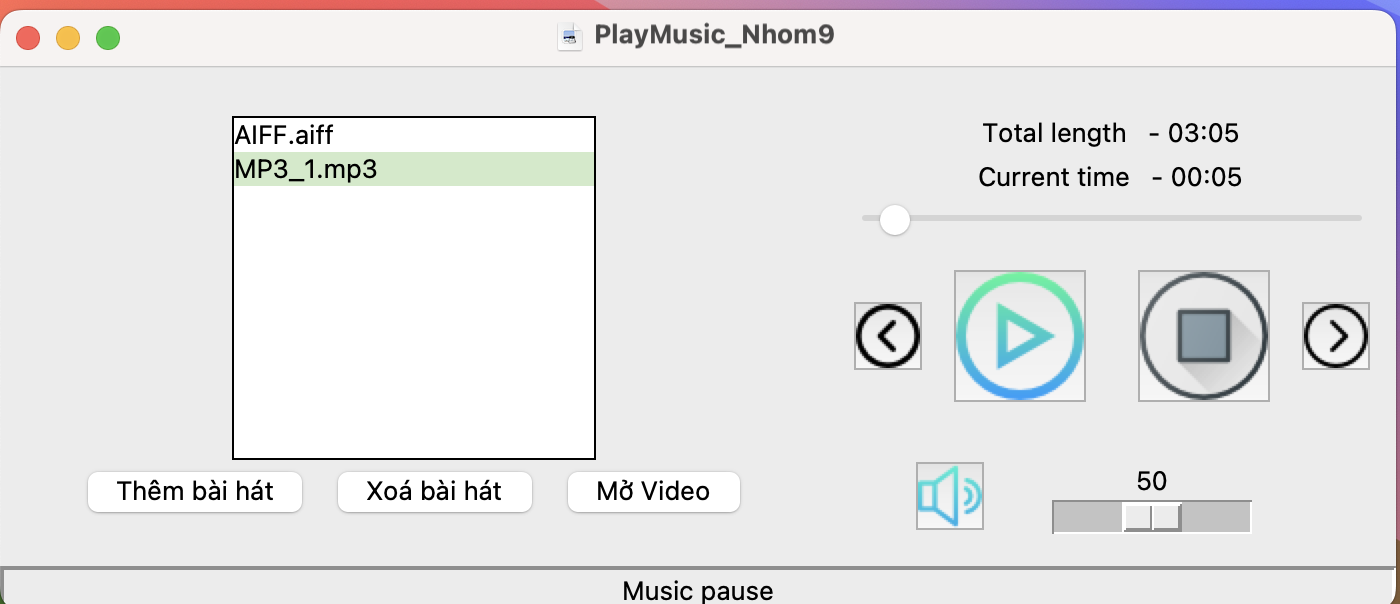
\includegraphics[width=130mm]{template_SGU 2/giaodien.png}
\end{center}
\begin{enumerate}
\item Thêm, xoá các bài hát vào danh sách phát và chọn video:
\begin{itemize}
    \item Bạn click vào nút thêm bài hát và lần lượt thêm các audio mà bạn yêu thích vào.
    \item Bạn chọn bài hát mà bạn không thích ở danh sách phát và bạn click vào nút "Xoá bài hát" để bạn xoá bài hát ra khỏi danh sách phát.
    \item Bạn click vào nút "Mở Video" và thực hiện chọn video có trên mấy mình để bắt đầu play chúng, khi bạn muốn tắt video bạn có thể ấn "q".
\end{itemize}
\item Play, pause, stop:
\begin{itemize}
    \item Sau khi bạn thêm được danh sách bài hát, bạn có thể ấn nút "Play" để bắt đầu play bài đầu tiên, hoặc bạn có thể chọn bài hát mà bạn muốn "Play" có trong danh sách phát và bắt đầu play nó.
    \item Bạn có thể tạm ngưng bài hát bằng cách ấn vào nút "Pause" và bắt chúng play tiếp tục bằng cách ấn vào nút play.
    \item Bạn có thể ngưng hoàn toàn bài hát bằng cách ấn vào nút "Stop".
\end{itemize}
\item Chuyển bài:
\begin{itemize}
    \item Bạn có thể chuyển bài xuống bằng cách ấn vào nút "Next".
    \item Bạn có thể chuyển bài xuống bằng cách ấn vào nút "Prever".
\end{itemize}
\item Điều chỉnh âm thanh, và vị trí đoạn nhạc:
\begin{itemize}
    \item Bạn có thể kéo tăng âm lượng hoặc giảm âm lượng bằng cách kéo lên xuống ở nút lên xuống âm lượng. Hoặc bạn có thể để âm lượng yêm lặng bằng cách ấn vào nút "mute".
    \item Bạn có thể điều chỉnh vị trí đoạn nhạc bằng cách kéo qua lại ở scroll chạy thời gian của đoạn nhạc.
\end{itemize}
\item Xử lý lỗi:
\begin{itemize}
    \item Nếu có bất kỳ lỗi nào xảy ra trong quá trình, các thông báo lỗi sẽ được hiển thị trong một cửa sổ pop-up.
\end{itemize}
\end{enumerate}

\newpage
%%%%%%%%%%%%%%%%%%%%%%%%%%%%%%%%%
\begin{thebibliography}{80}

\bibitem{py la gi}
Python Là Gì? Tất Tần Tật Về Ngôn Ngữ Lập Trình Python:
\href{https://s.net.vn/KIrI}{https://s.net.vn/KIrI}, truy cập ngày 28/4/2024.
\bibitem{py}
Python là gì? Các kiến thức cần biết về lập trình Python:
\href{https://s.net.vn/l8Eq}{https://s.net.vn/l8Eq}, truy cập ngày 28/4/2024.
\bibitem{py_tkinter}
Tkinter Python là gì? Tất cả những gì bạn cần biết về Tkinter:
\href{https://www.icantech.vn/kham-pha/tkinter}{https://www.icantech.vn/kham-pha/tkinter}, truy cập ngày 28/4/2024.
\end{thebibliography}
\end{document}

